% Options for packages loaded elsewhere
\PassOptionsToPackage{unicode}{hyperref}
\PassOptionsToPackage{hyphens}{url}
\PassOptionsToPackage{dvipsnames,svgnames,x11names}{xcolor}
%
\documentclass[
  man, donotrepeattitle,floatsintext]{apa7}
\usepackage{amsmath,amssymb}
\usepackage{lmodern}
\usepackage{iftex}
\ifPDFTeX
  \usepackage[T1]{fontenc}
  \usepackage[utf8]{inputenc}
  \usepackage{textcomp} % provide euro and other symbols
\else % if luatex or xetex
  \usepackage{unicode-math}
  \defaultfontfeatures{Scale=MatchLowercase}
  \defaultfontfeatures[\rmfamily]{Ligatures=TeX,Scale=1}
\fi
% Use upquote if available, for straight quotes in verbatim environments
\IfFileExists{upquote.sty}{\usepackage{upquote}}{}
\IfFileExists{microtype.sty}{% use microtype if available
  \usepackage[]{microtype}
  \UseMicrotypeSet[protrusion]{basicmath} % disable protrusion for tt fonts
}{}
\makeatletter
\@ifundefined{KOMAClassName}{% if non-KOMA class
  \IfFileExists{parskip.sty}{%
    \usepackage{parskip}
  }{% else
    \setlength{\parindent}{0pt}
    \setlength{\parskip}{6pt plus 2pt minus 1pt}}
}{% if KOMA class
  \KOMAoptions{parskip=half}}
\makeatother
\usepackage{xcolor}
\usepackage{graphicx}
\makeatletter
\def\maxwidth{\ifdim\Gin@nat@width>\linewidth\linewidth\else\Gin@nat@width\fi}
\def\maxheight{\ifdim\Gin@nat@height>\textheight\textheight\else\Gin@nat@height\fi}
\makeatother
% Scale images if necessary, so that they will not overflow the page
% margins by default, and it is still possible to overwrite the defaults
% using explicit options in \includegraphics[width, height, ...]{}
\setkeys{Gin}{width=\maxwidth,height=\maxheight,keepaspectratio}
% Set default figure placement to htbp
\makeatletter
\def\fps@figure{htbp}
\makeatother
\setlength{\emergencystretch}{3em} % prevent overfull lines
\providecommand{\tightlist}{%
  \setlength{\itemsep}{0pt}\setlength{\parskip}{0pt}}
\setcounter{secnumdepth}{-\maxdimen} % remove section numbering
% Make \paragraph and \subparagraph free-standing
\ifx\paragraph\undefined\else
  \let\oldparagraph\paragraph
  \renewcommand{\paragraph}[1]{\oldparagraph{#1}\mbox{}}
\fi
\ifx\subparagraph\undefined\else
  \let\oldsubparagraph\subparagraph
  \renewcommand{\subparagraph}[1]{\oldsubparagraph{#1}\mbox{}}
\fi
\newlength{\cslhangindent}
\setlength{\cslhangindent}{1.5em}
\newlength{\csllabelwidth}
\setlength{\csllabelwidth}{3em}
\newlength{\cslentryspacingunit} % times entry-spacing
\setlength{\cslentryspacingunit}{\parskip}
\newenvironment{CSLReferences}[2] % #1 hanging-ident, #2 entry spacing
 {% don't indent paragraphs
  \setlength{\parindent}{0pt}
  % turn on hanging indent if param 1 is 1
  \ifodd #1
  \let\oldpar\par
  \def\par{\hangindent=\cslhangindent\oldpar}
  \fi
  % set entry spacing
  \setlength{\parskip}{#2\cslentryspacingunit}
 }%
 {}
\usepackage{calc}
\newcommand{\CSLBlock}[1]{#1\hfill\break}
\newcommand{\CSLLeftMargin}[1]{\parbox[t]{\csllabelwidth}{#1}}
\newcommand{\CSLRightInline}[1]{\parbox[t]{\linewidth - \csllabelwidth}{#1}\break}
\newcommand{\CSLIndent}[1]{\hspace{\cslhangindent}#1}
\ifLuaTeX
\usepackage[bidi=basic]{babel}
\else
\usepackage[bidi=default]{babel}
\fi
\babelprovide[main,import]{english}
% get rid of language-specific shorthands (see #6817):
\let\LanguageShortHands\languageshorthands
\def\languageshorthands#1{}
% Manuscript styling
\usepackage{upgreek}
\captionsetup{font=singlespacing,justification=justified}

% Table formatting
\usepackage{longtable}
\usepackage{lscape}
% \usepackage[counterclockwise]{rotating}   % Landscape page setup for large tables
\usepackage{multirow}		% Table styling
\usepackage{tabularx}		% Control Column width
\usepackage[flushleft]{threeparttable}	% Allows for three part tables with a specified notes section
\usepackage{threeparttablex}            % Lets threeparttable work with longtable

% Create new environments so endfloat can handle them
% \newenvironment{ltable}
%   {\begin{landscape}\centering\begin{threeparttable}}
%   {\end{threeparttable}\end{landscape}}
\newenvironment{lltable}{\begin{landscape}\centering\begin{ThreePartTable}}{\end{ThreePartTable}\end{landscape}}

% Enables adjusting longtable caption width to table width
% Solution found at http://golatex.de/longtable-mit-caption-so-breit-wie-die-tabelle-t15767.html
\makeatletter
\newcommand\LastLTentrywidth{1em}
\newlength\longtablewidth
\setlength{\longtablewidth}{1in}
\newcommand{\getlongtablewidth}{\begingroup \ifcsname LT@\roman{LT@tables}\endcsname \global\longtablewidth=0pt \renewcommand{\LT@entry}[2]{\global\advance\longtablewidth by ##2\relax\gdef\LastLTentrywidth{##2}}\@nameuse{LT@\roman{LT@tables}} \fi \endgroup}

% \setlength{\parindent}{0.5in}
% \setlength{\parskip}{0pt plus 0pt minus 0pt}

% Overwrite redefinition of paragraph and subparagraph by the default LaTeX template
% See https://github.com/crsh/papaja/issues/292
\makeatletter
\renewcommand{\paragraph}{\@startsection{paragraph}{4}{\parindent}%
  {0\baselineskip \@plus 0.2ex \@minus 0.2ex}%
  {-1em}%
  {\normalfont\normalsize\bfseries\itshape\typesectitle}}

\renewcommand{\subparagraph}[1]{\@startsection{subparagraph}{5}{1em}%
  {0\baselineskip \@plus 0.2ex \@minus 0.2ex}%
  {-\z@\relax}%
  {\normalfont\normalsize\itshape\hspace{\parindent}{#1}\textit{\addperi}}{\relax}}
\makeatother

% \usepackage{etoolbox}
\makeatletter
\patchcmd{\HyOrg@maketitle}
  {\section{\normalfont\normalsize\abstractname}}
  {\section*{\normalfont\normalsize\abstractname}}
  {}{\typeout{Failed to patch abstract.}}
\patchcmd{\HyOrg@maketitle}
  {\section{\protect\normalfont{\@title}}}
  {\section*{\protect\normalfont{\@title}}}
  {}{\typeout{Failed to patch title.}}
\makeatother

\usepackage{xpatch}
\makeatletter
\xapptocmd\appendix
  {\xapptocmd\section
    {\addcontentsline{toc}{section}{\appendixname\ifoneappendix\else~\theappendix\fi\\: #1}}
    {}{\InnerPatchFailed}%
  }
{}{\PatchFailed}
\keywords{anecdotal bias, capital allocation, managerial decision-making, similarity\newline\indent Word count: 11117}
\usepackage{csquotes}
\raggedbottom
\renewcommand\author[1]{}
\renewcommand\affiliation[1]{}
\authorsnames[1, 1, 2]{Shir Dekel, Micah B. Goldwater, Dan Lovallo}
\authorsaffiliations{{The University of Sydney, School of Psychology}, {The University of Sydney, Business School}}
\usepackage{pdflscape}
\newcommand{\blandscape}{\begin{landscape}}
\newcommand{\elandscape}{\end{landscape}}
\ifLuaTeX
  \usepackage{selnolig}  % disable illegal ligatures
\fi
\IfFileExists{bookmark.sty}{\usepackage{bookmark}}{\usepackage{hyperref}}
\IfFileExists{xurl.sty}{\usepackage{xurl}}{} % add URL line breaks if available
\urlstyle{same} % disable monospaced font for URLs
\hypersetup{
  pdftitle={Anecdotal Bias in Allocation Decisions: The Role of Anecdote Similarity},
  pdfauthor={Shir Dekel1, Micah B. Goldwater1, \& Dan Lovallo2},
  pdflang={en-EN},
  pdfkeywords={anecdotal bias, capital allocation, managerial decision-making, similarity},
  colorlinks=true,
  linkcolor={NavyBlue},
  filecolor={Maroon},
  citecolor={Blue},
  urlcolor={Blue},
  pdfcreator={LaTeX via pandoc}}

\title{Anecdotal Bias in Allocation Decisions: The Role of Anecdote Similarity}
\author{Shir Dekel\textsuperscript{1}, Micah B. Goldwater\textsuperscript{1}, \& Dan Lovallo\textsuperscript{2}}
\date{}


\shorttitle{Anecdotal Bias in Allocation Decisions}

\authornote{

Shir Dekel \url{https://orcid.org/0000-0003-1773-2446}.

Micah B. Goldwater \url{https://orcid.org/0000-0001-8052-9497}.

Portions of this work comprised Shir Dekel's doctoral dissertation.

All data, analysis code, and research materials are available at
\url{https://github.com/shirdekel/anecdotal-bias-in-allocation-decisions}.

Correspondence concerning this article should be addressed to Shir Dekel, Brennan MacCallum Building (A18) Camperdown, NSW 2006, Australia. E-mail: \href{mailto:shir.dekel@sydney.edu.au}{\nolinkurl{shir.dekel@sydney.edu.au}}

}

\affiliation{\vspace{0.5cm}\textsuperscript{1} The University of Sydney, School of Psychology\\\textsuperscript{2} The University of Sydney, Business School}

\abstract{%
Both anecdotes and aggregated data impact decision-making but it
is unclear how the two are integrated when making decisions. Typically, it is
normative to focus on aggregated data over an anecdote when the two appear in
conflict. However, the similarity of each data point to the target problem is
also important because a highly similar anecdote may be more informative than
the rest of the cases in the data. The present study is the first to investigate
whether people's decisions are influenced by the similarity of an anecdote to
the target problem while considering the similarity of the anecdote to the other
cases within the aggregated data. When reasoning with both anecdotes and
aggregated data, the results show that anecdotes influence participants'
decisions only when they are similar to the target problem. However, when
participants were given information about the equivalent similarity between the
anecdote and the cases in the larger set of data, they showed the same pattern
of anecdotal influence as when they had no such information. Therefore, people
seem to appropriately use an anecdote from a set of cases based on its
similarity to the target case, but do not understand the importance of its
similarity to the other cases in the set.
}



\usepackage{amsthm}
\newtheorem{theorem}{Theorem}
\newtheorem{lemma}{Lemma}
\newtheorem{corollary}{Corollary}
\newtheorem{proposition}{Proposition}
\newtheorem{conjecture}{Conjecture}
\theoremstyle{definition}
\newtheorem{definition}{Definition}
\theoremstyle{definition}
\newtheorem{example}{Example}
\theoremstyle{definition}
\newtheorem{exercise}{Exercise}
\theoremstyle{definition}
\newtheorem{hypothesis}{Hypothesis}
\theoremstyle{remark}
\newtheorem*{remark}{Remark}
\newtheorem*{solution}{Solution}
\begin{document}
\maketitle



















\hypertarget{anecdotal-bias-in-capital-allocation-depends-on-anecdote-similarity}{%
\section{Anecdotal Bias in Capital Allocation Depends on Anecdote Similarity}\label{anecdotal-bias-in-capital-allocation-depends-on-anecdote-similarity}}

A good story is often more persuasive than data. While usually harmless in daily
settings, poor judgement arising from a bias towards anecdotal evidence can lead
to large-scale negative consequences. Perhaps the most prominent example of such
an error in judgement is the belief that a vaccine causes a certain disorder
based on isolated stories, despite contradictory scientific evidence. An
analogous error exists in settings such as managerial decision-making. This is a
domain that is useful to study this bias because in business, managers use
analogies, known as \emph{case studies}, as a part of their strategic
decision-making. Case studies are examples of previous situations considered
similar by the decision-maker and are used to draw inferences about a target
problem (\protect\hyperlink{ref-gavetti2005}{Gavetti et al., 2005}; \protect\hyperlink{ref-gavetti2005a}{Gavetti \& Rivkin, 2005}). Case studies are known as \emph{anecdotes}
when comparing them with aggregated data. It is unclear how people balance the
use of anecdotes and aggregated data in these settings.

Many businesses use case studies to inform their decisions but often struggle to
use them properly (\protect\hyperlink{ref-gavetti2005a}{Gavetti \& Rivkin, 2005}). This may be attributable to the prominence of
companies that are either highly successful or highly unsuccessful. That is,
people are often uninterested in average outcomes but are captivated by both
positive and negative extreme outcomes. The increased salience of an anecdote
may increase its influence over that of useful statistical data. Further,
increased anecdotal salience may also shift attention away from relational
similarities most relevant to understanding the underlying causes of success and
failure in the case studies in favour of more surface similarities between an
anecdote and current problem. Both issues may explain the improper use of case
studies.

The first consideration when using a case study is its merit relative to
available aggregated statistical data. That is, if the case study is a single
data point in a set of other equally relevant cases, then using the statistical
properties of the larger sample is more inferentially informative than using a
single case from within the sample (unlike perhaps when the single case is
somehow the most relevant example from the sample). Despite the utility and
availability of large sample data, research has shown that people often prefer
anecdotal evidence over statistical data (\protect\hyperlink{ref-freling2020}{Freling et al., 2020}; \protect\hyperlink{ref-jaramillo2019}{Jaramillo et al., 2019}; \protect\hyperlink{ref-reinard1988}{Reinard, 1988}; \protect\hyperlink{ref-shen2015}{Shen et al., 2015}).

However, if this larger sample is not available (or is ignored), then the second
consideration when using a case study is the extent of its similarity to the
target problem. Research on the psychology of similarity judgements
distinguishes between surface and relational similarity (e.g., \protect\hyperlink{ref-gentner1983}{Gentner, 1983}).
The consensus of this research is that the more conceptual structures that two
cases share, the more useful they are in decision-making (\protect\hyperlink{ref-lassaline1996}{Lassaline, 1996}; \protect\hyperlink{ref-markman1995}{Markman \& Medin, 1995}). Therefore, case studies that are similar to a target problem on
a merely surface level are less useful than those that are related through a
shared conceptual structure.

Previous research has considered the role of similarity and analogical reasoning
in business-related decision-making (e.g., \protect\hyperlink{ref-gavetti2005}{Gavetti et al., 2005}; \protect\hyperlink{ref-lovallo2012}{Lovallo et al., 2012}). Others
have investigated the influence of anecdotes in capital allocation decisions and
the impact of anecdote similarity on their persuasiveness (summarised below).
Capital allocation is the process of distributing money within an organisation
and offers a useful paradigm to study anecdotes and similarity. Case studies are
important in capital allocation because that is how decisions are often
presented to executives. Further, anecdote similarity is an important factor in
capital allocation because business unit functions within a firm can be quite
unrelated. For instance, two of General Electric's divisions include GE Aviation
and GE Healthcare. This such a firm may rely more on cases from other companies
to compare to their projects. However, it is unclear to what extent an
anecdote's similarity to the target problem will affect its influence on capital
allocation decisions. Also it is unclear if this effect would depend on whether
the anecdote is of a successful or unsuccessful case (anecdote valence). Recent
evidence from medical decision-making suggests negative anecdotes have greater
effect (\protect\hyperlink{ref-jaramillo2019}{Jaramillo et al., 2019}). Further, when balancing the use of aggregated data and
an anecdote, it is unclear whether people will be sensitive to information about
the distribution of the aggregated data from which the anecdote was sampled.
Normative use of anecdotes would consider this information.

Therefore, we considered three novel questions: (a) does the anecdotal bias
effect depend on the similarity of the anecdote to the target project? (b) Do
people consider verbal sample distribution information to help inform their
decisions? And (c) is the magnitude of this effect different between negative
and positive anecdotes?

\hypertarget{anecdotal-bias}{%
\subsection{Anecdotal Bias}\label{anecdotal-bias}}

Anecdotal bias refers to the over-weighting of anecdotal evidence as compared to
statistical evidence on people's beliefs. Journalists, for instance, are well
aware of the power of anecdotes. An analysis of approximately 29,000 New York
Times editorials showed a reliance on anecdotes to drive arguments
(\protect\hyperlink{ref-alkhatib2017}{Al Khatib et al., 2017}). While some studies have concluded that statistics are more
persuasive than anecdotes (e.g., \protect\hyperlink{ref-allen1997}{Allen \& Preiss, 1997}; \protect\hyperlink{ref-hoeken2001}{Hoeken, 2001}; \protect\hyperlink{ref-hornikx2005}{Hornikx, 2005}) and
others provided more cautious conclusions (\protect\hyperlink{ref-winterbottom2008}{Winterbottom et al., 2008}), a number have
found evidence for anecdotal bias (e.g., \protect\hyperlink{ref-jaramillo2019}{Jaramillo et al., 2019}; \protect\hyperlink{ref-ratcliff2020}{Ratcliff \& Sun, 2020}; \protect\hyperlink{ref-reinard1988}{Reinard, 1988}; \protect\hyperlink{ref-reinhart2006}{Reinhart, 2006}; \protect\hyperlink{ref-shen2015}{Shen et al., 2015}). Zebregs et al. (\protect\hyperlink{ref-zebregs2015}{2015}) suggest that this
disparity in findings might be attributable to statistics affecting beliefs and
attitudes, and anecdotes affecting intention. A more recent meta-analysis of 61
studies found that, overall, statistical evidence is more persuasive than
anecdotal evidence (\protect\hyperlink{ref-freling2020}{Freling et al., 2020}). However, this advantage for statistics may be
due to experimental methods where participants are presented with situations to
evaluate that have no direct relevance to their lives. The meta-analysis found
that people tend to prefer anecdotal evidence over statistical data when the
stakes are more emotional, medical, or relevant to the decision-maker. In
business, decisions are clearly relevant to the decision-maker because they can
mean the difference between a promotion or getting fired. Even so, experimental
research shows that anecdotes that add no additional information to co-presented
statistics may still influence people's judgement, and further show that all
anecdotes are not created equal in how they affect judgments (e.g., \protect\hyperlink{ref-jaramillo2019}{Jaramillo et al., 2019}). This suggests experimental methods, such as those used in the
current research, are still appropriate to identify how anecdotes influences
judgment, and if anything, \emph{under-estimate} the size of the effect in the
real-world where people consider decisions relevant to themselves.

\hypertarget{anecdotal-bias-in-business}{%
\subsection{Anecdotal Bias in Business}\label{anecdotal-bias-in-business}}

It is important to investigate anecdotal bias in business contexts because of
its implications for managers' use of similar ``comparables'' when making
strategic decisions. There are many cases of managers successfully using
analogies from anecdotal cases but also of failures to analogise correctly
(\protect\hyperlink{ref-gavetti2005}{Gavetti et al., 2005}; \protect\hyperlink{ref-gavetti2005a}{Gavetti \& Rivkin, 2005}). There is very little experimental research on
anecdotal bias in business, but the existing work finds clear evidence of the
effect.

Wainberg et al. (\protect\hyperlink{ref-wainberg2013}{2013}) gave a sample of managers and other professionals a choice between
two audit firms, which varied in terms of their audit deficiencies for various
clients. The experiment was designed in such a way that the statistical evidence
favoured one firm, while the anecdotal evidence favoured the other firm.
Participants in the \emph{anecdotes only} condition were given anecdotal examples of
firm deficiencies, while those in the \emph{anecdotes \& statistics} condition were
given the same anecdotal examples as well as the number of clients and
deficiencies found and the proportions of these values.\footnote{This condition is referred to as anecdotes \& enhanced
  statistics in (\protect\hyperlink{ref-wainberg2013}{Wainberg et al., 2013}) but was changed to anecdotes \& statistics here for
  clarity. Their ``anecdotes and statistics'' condition had less statistical
  information and we decided to just use the condition that had more information.}
Participants in the \emph{statistics only} condition were given this proportions
information as well as the number of clients without deficiencies but no
detailed examples of deficiencies.

Wainberg et al. (\protect\hyperlink{ref-wainberg2013}{2013}) measured the percentage of participants who chose firms favoured
by the statistical data, finding evidence of anecdotal bias. Participants in the
anecdotes \& statistics condition were less likely to choose the firm favoured by
statistical data compared with those in the statistics only condition. This
shows evidence of anecdotal bias because participants ignored contradictory
statistical data. They also found a difference between the anecdotes \&
statistics condition and the anecdotes only condition, which implies that the
anecdotal bias effect was ``partial''. That is, the presented statistics played
some role in influencing participants' choice of firm. A ``complete'' effect would
have occurred if there was no difference between the conditions, meaning that
statistics would have not played a role in influencing choice.

The other important finding in this work is that anecdotal bias was reduced by
highlighting relevant statistical features and providing an explanation of
statistical inference. This is important because it suggests that potential
psychological biases can be reduced with a reframing of provided information and
an explanation of relevant statistical concepts.

Wainberg (\protect\hyperlink{ref-wainberg2018}{2018}) conducted a similar study to that of Wainberg et al. (\protect\hyperlink{ref-wainberg2013}{2013}) but with a
capital budgeting task as opposed to a binary choice. Participants had to choose
between three production line machines for a mid-sized company that prints
circuit boards. The statistical data suggested that Machine~A was better than
Machine~B, and Machine~B was better than Machine~C. Participants were given only
statistical information or statistical information along with an anecdote. The
anecdote was in the form of an email from a colleague who recommended against
Machine~A (the best option). Similar to Wainberg et al. (\protect\hyperlink{ref-wainberg2013}{2013}), participants were
assigned to \emph{anecdote \& statistics} and \emph{statistics only} conditions. In another
condition, participants were told to ``think like a scientist'' and received an
explanation of the importance of statistical inference.

Wainberg (\protect\hyperlink{ref-wainberg2018}{2018}) found evidence for anecdotal bias. Including a contradictory
anecdote alongside statistical evidence (the anecdote \& statistics condition)
reduced the proportion of participants who chose Machine~A. The study also found
that the addition of instructions that emphasised scientific thinking reduced
this bias. Unlike Wainberg et al. (\protect\hyperlink{ref-wainberg2013}{2013}), Wainberg (\protect\hyperlink{ref-wainberg2018}{2018}) could not determine whether the
anecdotal bias was complete or partial because there was no anecdote only
condition. Further, neither work considered the effect of the anecdote's
similarity to the target problem, nor whether this similarity differed to that
of the other cases in the aggregated data set. In the present study we test an
anecdote only condition, consider the anecdote's similarity to the target
problem, and investigate whether participants are sensitive to information about
the distribution of similarity in the aggregated data.

\hypertarget{effect-of-similarity}{%
\subsection{Effect of Similarity}\label{effect-of-similarity}}

Arguably, the extent of one's reliance on an anecdote should depend on its
similarity to the target problem. Previous work has examined the importance of
weighting previous cases according to their similarity to the present situation
(\protect\hyperlink{ref-gilboa1995}{Gilboa \& Schmeidler, 1995}; \protect\hyperlink{ref-lovallo2012}{Lovallo et al., 2012}). For instance, consider a medical treatment with
contradictory statistical and anecdotal evidence; that is, a large-scale
aggregated study has found that the treatment has 99\% efficacy, while someone
reports on social media that they became sick as a side-effect of the treatment.
While the decision to use the treatment should be informed more by the
aggregated data than by the anecdotal data, an individual may have reason to be
concerned if the person who became sick was their identical twin. Therefore, the
inference that the individual may also need to be cautious about the treatment
arises from a specific causal model based on the shared genetics of the two
cases.

There have been mixed results regarding the effect of anecdote similarity on
people's use of anecdotes. Hoeken and Hustinx (\protect\hyperlink{ref-hoeken2009}{2009}, Study~3) found evidence for the effect
of similarity on the persuasiveness of a variety of anecdotes. As well as
manipulating whether participants received a claim supported by anecdotal or
statistical evidence, they manipulated whether the anecdotal evidence was
similar or dissimilar to the claim that it was supporting. They found that
similar anecdotes were more persuasive than dissimilar anecdotes. Using a
student sample, Hoeken (\protect\hyperlink{ref-hoeken2001}{2001}) did not find evidence for the effect of similarity
to a local government proposal. Similarly, Hornikx (\protect\hyperlink{ref-hornikx2018}{2018}) considered the effect of
similarity on anecdotal bias in local government policy decision-making. The
researchers did not find an effect for similarity or for anecdotes. However,
they measured persuasiveness, whereas concrete allocation of funds may better
show the influence of anecdotes. Further, the content of all the anecdotes that
both Hoeken and Hornikx presented their participants was the same. Therefore, it
is unclear if their lack of similarity effect was due to the specific scenario
participants were presented. The present study clarifies this by testing a
similarity effect with concrete decisions and multiple anecdote domains.

Apart from the need to determine the effect of similarity on the anecdotal bias
effect, it is important to clarify how such an effect might work. Research on
analogical reasoning has distinguished between simple surface similarity and
deeper relational similarity (\protect\hyperlink{ref-gentner1983}{Gentner, 1983}). As mentioned above, one's use of
an anecdote should depend on the extent to which it is associated by an
underlying causal mechanism relevant to the target problem or mere surface
similarity. Imagine a manager of a multi-divisional company deciding on the
allocation of capital between an oil well project and a technology project.
Would hearing of a recent failed oil well project at another company influence
the manager's allocation decision? If so, would it influence the manager's
decision because the anecdote has similarities to the target oil well project
(surface similarity)? Or would the manager seek out the underlying reason for
the failure of the other company's oil well project to identify whether it is
relevant to the target oil project (relational similarity)? The experiments
presented in this study investigated whether the anecdotal bias effect arose
from causal inductive reasoning or merely the surface similarity with the target
project. This distinction may help address the mixed findings mentioned above,
as it is unclear if the previous studies manipulated surface or relational
similarity. Often, ``anecdotal thinking'' is a pejorative term, assuming it is
unsophisticated and superficial. However, if the use of anecdotes is based on
shared underlying causal mechanisms, and considers the relative similarity of
the anecdote to the distribution of cases the anecdote is a part of, then this
suggests a more sophisticated way of thinking (\protect\hyperlink{ref-gavetti2005}{Gavetti et al., 2005}).

\hypertarget{experiment-summary}{%
\subsection{Experiment Summary}\label{experiment-summary}}

Experiment~1 investigates whether people are sensitive to the similarity of an
anecdote to the target problem. Further, it tests whether providing participants
with simple instructions will encourage them to aggregated data over an
anecdote. In Experiment~2 we tell participants that the anecdote is as similar
to the target problem as the rest of the aggregated data to see if they
correctly disregard it. Previous research suggests that people may respond
differently to a negative anecdote, which is an example of an unsuccessful case,
compared to a positive anecdote, which is an example of a successful case. In
line with this, Experiment~1 only uses negative anecdotes. However, Experiment~2
further examines this distinction by contrasting positive with negative
anecdotes.

\hypertarget{anecdotes-1}{%
\section{Experiment~1}\label{anecdotes-1}}

Experiment~1 investigated the effects of anecdote similarity and bias on capital
allocation. Participants were assigned to the anecdote \& statistics and
statistics only conditions as in Wainberg (\protect\hyperlink{ref-wainberg2018}{2018}), with an addition of an anecdote
only condition. They were then asked to allocate a hypothetical budget between
two business projects. Participants were also presented with a case study that
was either similar or less similar to the target project, which Wainberg did not
do. Note, however, that a less similar project here is still significantly
related to the target project because they are both from the same industry.
Further, for the conditions in which statistical evidence was provided,
participants were presented with aggregated information about the success of
similar projects in the form of Net Present Value (NPV)\footnote{\[
  \text{NPV}=\sum_{t=0}^n \frac{R_t}{(1+i)^t},
  \]

  where \(t\) is the time of the cash flow, \(i\) is the discount rate, \(R_t\) is the
  net cash flow, and \(n\) is the total number of periods.} as well as a
reliability measure. NPV is the difference between the forecasted revenue of a
project and the initial investment in its development (accounting for the time
value of money), and was chosen here because it is the most common financial
measure that is used by executives in order to value business project proposals
(\protect\hyperlink{ref-graham2015}{Graham et al., 2015}; \protect\hyperlink{ref-graham2001}{Graham \& Harvey, 2001}; \protect\hyperlink{ref-remer1993}{Remer et al., 1993}). One project was clearly better than the
other in terms of the statistical data, but the anecdotal evidence suggested the
opposite.

Previous research has found that people are persuaded more by negative anecdotes
than by positive statistical data in capital allocation scenarios
(\protect\hyperlink{ref-wainberg2018}{Wainberg, 2018}). While studies have shown that similar anecdotes are more
persuasive than dissimilar anecdotes (\protect\hyperlink{ref-hoeken2009}{Hoeken \& Hustinx, 2009}; Study~3), it is unclear how
the anecdotal bias effect may depend on anecdote similarity. That is, it is
unclear whether people will respond to a simple negative association of the
anecdote to the target, or use a more sophisticated causal induction. The
present study is novel because we investigate both anecdotal bias and anecdotal
similarity. This is different from Hoeken and Hustinx because we presented
participants aggregated data to investigate anecdotal bias, whereas Hoeken and
Hustinx only presented anecdotes. Thus, the main question is whether anecdotal
bias will be greater when the anecdote is similar to the target project compared
with when it is less similar. The target project is supported by the statistics
but is inconsistent with the anecdotes. Further, Experiment~1 only uses negative
anecdotes. Therefore, the experiment would show evidence of anecdotal bias if
participants assigned to the statistics only condition allocated more money to
the target project compared with those in the anecdote \& statistics condition.
Therefore, Experiment~1 tests the following hypothesis:

\begin{hypothesis}[anecdotal bias depends on the similarity of negative anecdotes]
\protect\hypertarget{hyp:anecdote-similarity-anecdotes-1}{}\label{hyp:anecdote-similarity-anecdotes-1}Budget allocations to the target project will be higher when statistics only are
presented compared with when statistics are accompanied by an anecdote with high
similarity to the target project. In addition, budget allocations will not be
affected by anecdotes with low similarity. That is, the statistics only
condition will not differ from the low-similarity anecdote \& statistics
condition.
\end{hypothesis}

We predict that that the anecdotal bias effect will be partial. Specifically,
the participants presented with the high-similarity anecdote along with the
statistics would use some of the statistical information. Testing the high
similarity condition will provide an equivalent test to that of Wainberg et al. (\protect\hyperlink{ref-wainberg2013}{2013}).
Therefore, Experiment~1 tests the following:

\begin{hypothesis}[effect of statistics for negative anecdotes]
\protect\hypertarget{hyp:statistics-anecdotes-1}{}\label{hyp:statistics-anecdotes-1}Participants in the high-similarity anecdote \& statistics condition (without the
enhanced statistics explanation) will allocate more capital to the target
project than those in the high-similarity anecdote only condition.
\end{hypothesis}

In a condition we refer to as the anecdote \& enhanced statistics condition,
participants were provided with additional information about the importance of
scientific thinking and statistical data. The statistics here are enhanced
because participants were provided with information that should help them better
interpret the statistics and therefore may be less affected by anecdotes.
Experiment~1 tests whether the effect of additional information on anecdotal
bias found in Wainberg (\protect\hyperlink{ref-wainberg2018}{2018}) would be replicated in a capital allocation
scenario. Therefore, Experiment~1 tests the following hypothesis:

\begin{hypothesis}[effect of enhanced statistics for negative anecdotes]
\protect\hypertarget{hyp:enhanced-statistics-anecdotes-1}{}\label{hyp:enhanced-statistics-anecdotes-1}Participants in the high-similarity anecdote \& enhanced statistics condition
will allocate more capital to the target project than those in the
high-similarity anecdote \& statistics condition.
\end{hypothesis}

\hypertarget{method-1}{%
\subsection{Method}\label{method-1}}

\hypertarget{transparency-and-openness}{%
\subsubsection{Transparency and openness}\label{transparency-and-openness}}

We report how we determined our sample size, all data exclusions, all
manipulations, and all measures in the study. All data, analysis code, and
research materials are available at
\url{https://github.com/shirdekel/anecdotal-bias-in-allocation-decisions}
(\protect\hyperlink{ref-dekel2022}{Dekel, 2022a}). This study's design and its analysis were not pre-registered. The
article used R (Version 4.2.0; \protect\hyperlink{ref-R-base}{R Core Team, 2022}) \footnote{We, furthermore, used the R-packages \emph{afex} (Version 1.2.0; \protect\hyperlink{ref-R-afex}{Singmann et al., n.d.}), \emph{anecdotes1} (Version 1.0; \protect\hyperlink{ref-R-anecdotes1}{Dekel, 2021}), \emph{anecdotes2} (Version 1.0; \protect\hyperlink{ref-R-anecdotes2}{Dekel, 2022b}), \emph{bookdown} (Version 0.26; \protect\hyperlink{ref-R-bookdown}{Xie, 2016}), \emph{broom} (Version 0.8.0; \protect\hyperlink{ref-R-broom}{Robinson et al., 2022}), \emph{conflicted} (Version 1.1.0; \protect\hyperlink{ref-R-conflicted}{Wickham, 2021a}), \emph{dotenv} (Version 1.0.3; \protect\hyperlink{ref-R-dotenv}{Csárdi, 2021}), \emph{dplyr} (Version 1.0.9; \protect\hyperlink{ref-R-dplyr}{Wickham et al., 2022}), \emph{effectsize} (Version 0.6.0.1; \protect\hyperlink{ref-R-effectsize}{Ben-Shachar et al., 2020}), \emph{emmeans} (Version 1.7.4.1; \protect\hyperlink{ref-R-emmeans}{Lenth, 2022}), \emph{forcats} (Version 0.5.1; \protect\hyperlink{ref-R-forcats}{Wickham, 2021b}), \emph{Formula} (Version 1.2.4; \protect\hyperlink{ref-R-Formula}{Zeileis \& Croissant, 2010}), \emph{ggbeeswarm} (Version 0.6.0; \protect\hyperlink{ref-R-ggbeeswarm}{Clarke \& Sherrill-Mix, 2017}), \emph{ggplot2} (Version 3.3.6; \protect\hyperlink{ref-R-ggplot2}{Wickham, 2016}), \emph{here} (Version 1.0.1; \protect\hyperlink{ref-R-here}{Müller, 2020}), \emph{Hmisc} (Version 4.7.0; \protect\hyperlink{ref-R-Hmisc}{Harrell Jr, 2022}), \emph{janitor} (Version 2.1.0; \protect\hyperlink{ref-R-janitor}{Firke, 2021}), \emph{knitr} (Version 1.39; \protect\hyperlink{ref-R-knitr}{Xie, 2015}), \emph{lattice} (Version 0.20.45; \protect\hyperlink{ref-R-lattice}{Sarkar, 2008}), \emph{lme4} (Version 1.1.29; \protect\hyperlink{ref-R-lme4}{Bates et al., 2015}), \emph{magick} (Version 2.7.3; \protect\hyperlink{ref-R-magick}{Ooms, 2021}), \emph{magrittr} (Version 2.0.3; \protect\hyperlink{ref-R-magrittr}{Bache \& Wickham, 2022}), \emph{Matrix} (Version 1.4.1; \protect\hyperlink{ref-R-Matrix}{Bates et al., 2022}), \emph{papaja} (Version 0.1.0.9999; \protect\hyperlink{ref-R-papaja}{Aust \& Barth, 2022}), \emph{purrr} (Version 0.3.4; \protect\hyperlink{ref-R-purrr}{Henry \& Wickham, 2020}), \emph{rlang} (Version 1.0.2; \protect\hyperlink{ref-R-rlang}{Henry \& Wickham, 2022}), \emph{scales} (Version 1.2.0; \protect\hyperlink{ref-R-scales}{Wickham \& Seidel, 2022}), \emph{snakecase} (Version 0.11.0; \protect\hyperlink{ref-R-snakecase}{Grosser, 2019}), \emph{stringr} (Version 1.4.0; \protect\hyperlink{ref-R-stringr}{Wickham, 2019}), \emph{survival} (Version 3.3.1; \protect\hyperlink{ref-R-survival-book}{Terry M. Therneau \& Patricia M. Grambsch, 2000}), \emph{tarchetypes} (Version 0.6.0; \protect\hyperlink{ref-R-tarchetypes}{Landau, 2021a}), \emph{targets} (Version 0.12.0; \protect\hyperlink{ref-R-targets}{Landau, 2021b}), \emph{tidyr} (Version 1.2.0; \protect\hyperlink{ref-R-tidyr}{Wickham \& Girlich, 2022}), \emph{tinylabels} (Version 0.2.3; \protect\hyperlink{ref-R-tinylabels}{Barth, 2022}), and \emph{yaml} (Version 2.3.5; \protect\hyperlink{ref-R-yaml}{Garbett et al., 2022}).} to analyse and
plot the data, generate the experimental materials, and compile the document
itself. This study received approval by The University of Sydney Human Research
Ethics Committee (HREC; Project No.: 2019/056).

\hypertarget{participants}{%
\subsubsection{Participants}\label{participants}}

Two hundred and eighty-four participants (197 female) were recruited from a cohort of psychology undergraduates at The University of Sydney. Participants were compensated with course credit. The average age was 20.84 years (\emph{SD} = 4.93, \emph{min.} = 18, \emph{max.} = 58). Participants reported an average of 1.68 years (\emph{SD} = 3.63, \emph{min.} = 0, \emph{max.} = 32) working in a business setting, and an average of 0.81 years (\emph{SD} = 1.57, \emph{min.} = 0, \emph{max.} = 12) of business education. The mean completion time of the task was 22.24 min.~Three participants were removed from the data because
they reported being younger than 18.
Table~\ref{tab:condition-allocation-1} shows the allocation of
participants to the different conditions.
Appendix~\ref{power-analysis-1} describes the power analysis
conducted to arrive at this sample size.

\begin{table}[tbp]

\begin{center}
\begin{threeparttable}

\caption{\label{tab:condition-allocation-1}Experiment 1 group allocation.}

\begin{tabular}{lll}
\toprule
Evidence type & \multicolumn{1}{c}{Project alignment} & \multicolumn{1}{c}{N}\\
\midrule
Anecdote \& enhanced statistics & High & 41\\
Anecdote \& enhanced statistics & Low & 41\\
Anecdote \& statistics & High & 41\\
Anecdote \& statistics & Low & 40\\
Anecdote only & High & 41\\
Anecdote only & Low & 40\\
Statistics only & NA & 40\\
Total &  & 284\\
\bottomrule
\end{tabular}

\end{threeparttable}
\end{center}

\end{table}

\hypertarget{materials-1}{%
\subsubsection{Materials}\label{materials-1}}

\hypertarget{instructions-materials-1}{%
\paragraph{Instructions}\label{instructions-materials-1}}

All participants were first shown general instructions explaining the task.
Subsequent instructions shown to participants depended on their experimental
condition. Those in the anecdote only condition were told that they would be
shown a case study of a failed project and an analysis of why it failed. Those
in the statistics only condition were told that they would be shown NPV and
reliability information for two focal projects. They were told that these values
were sourced from a study with a large sample. Those in the anecdote \&
statistics condition were shown both of these instructions and were also told
that the information in the anecdote had been included in the aggregated study
data. Those in the anecdote \& enhanced statistics condition were shown the same
instructions as those in the anecdote \& statistics condition, but were also
provided with the explanation of scientific thinking used by Wainberg (\protect\hyperlink{ref-wainberg2018}{2018}).
Appendix~\ref{instructions-materials-1-appendix} shows the
instructions used in Experiment~1.

\hypertarget{allocation-task}{%
\paragraph{Allocation Task}\label{allocation-task}}

In the allocation task, participants were asked to allocate a hypothetical
budget to one of two projects from two different businesses. In this study,
these projects are referred to as the \emph{focal} projects, with one being the
\emph{target} project and the other the \emph{comparison} project. The target project was
used as the reference for the similarity manipulation. That is, the anecdote was
either high or low in similarity to the target project. Further, the data
analyses presented in the Results section used allocations to the target project
as the dependent variable. The comparison project was simply the other focal
project to which participants were allocating. It was a different type of
project to both the target and anecdote projects and was the same for all
participants.

Participants were presented with information about the name, location,
integration (vertical or horizontal)\footnote{A horizontally integrated company is one which is made up of
  multiple businesses that operate in similar markets, and may have previously
  been competitors (\protect\hyperlink{ref-gaughan2012}{Gaughan, 2012a}). A vertically integrated company, on the other
  hand, is one which is made up of multiple business than operate in the same
  market, but in different levels of the supply chain (\protect\hyperlink{ref-gaughan2012a}{Gaughan, 2012b}).}, and organisational structure
(centralised or decentralised)\footnote{A centralised organisational structure is one in which a company
  decisions tend to come from a specific business unit or leader, whereas a
  decentralised structure is one in which decisions can be made by separate units
  or people independently (\protect\hyperlink{ref-kenton2021}{Kenton, 2021}).} of each business. Further, they were
presented with information about the features of each project that are typically
available to managers prior to investment. Participants in the anecdote only
condition were shown only this information (see
Figure~\ref{fig:allocation-anecdote-only-1}). Those
in the anecdote \& statistics, anecdote \& enhanced statistics, and statistics
only conditions were shown this information along with measures of NPV and
overall reliability rating (see
Figure~\ref{fig:allocation-statistics-1}). The
overall reliability rating was created for the purpose of the experiment and
always varied alongside NPV. That is, overall reliability rating and NPV for the
target project were always both either higher or lower than the comparison
project. Participants entered their allocation data beneath this table in two
text boxes labelled \emph{Project~A allocation} and \emph{Project~B allocation},
respectively.



\begin{figure}
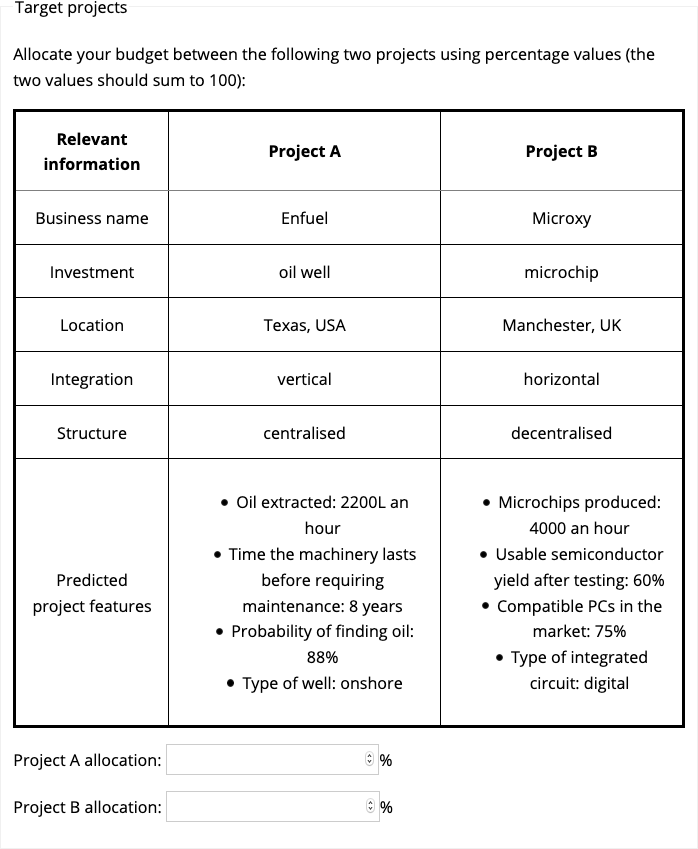
\includegraphics[width=1\linewidth]{anecdotal-bias-in-allocation-decisions_files/figure-latex/allocation-anecdote-only-1-1} \caption{Focal project display for the anecdote only condition in Experiment~1. Here, Project~A was the target project and Project~B was the comparison project.}\label{fig:allocation-anecdote-only-1}
\end{figure}



\begin{figure}
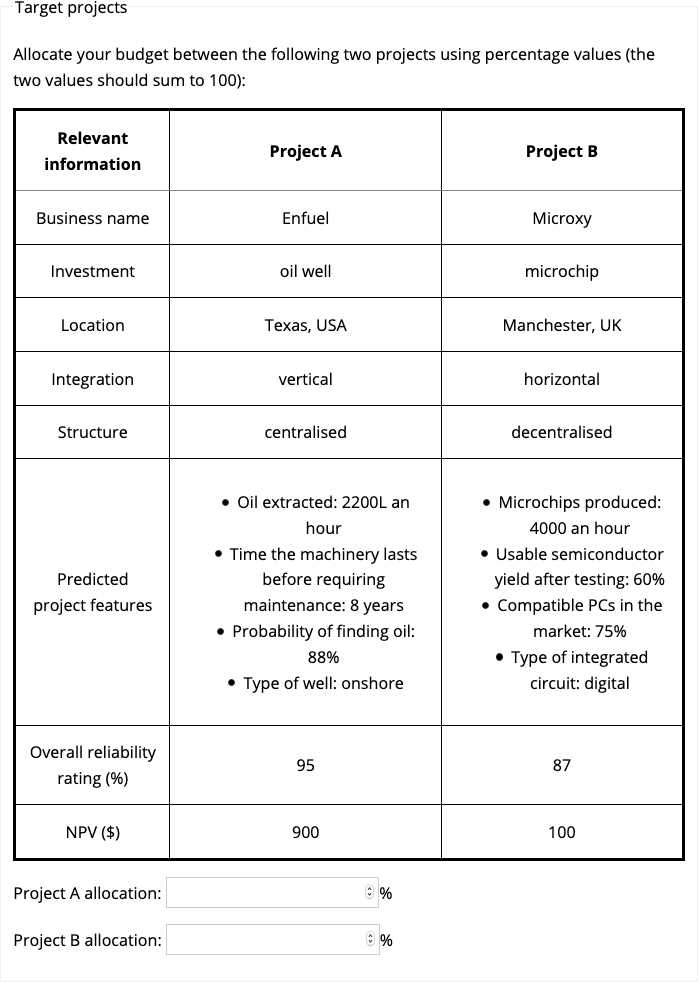
\includegraphics[width=0.95\linewidth]{anecdotal-bias-in-allocation-decisions_files/figure-latex/allocation-statistics-1-1} \caption{Focal project display for the statistics only, anecdote \& statistics, and anecdote \& enhanced statistics conditions in Experiment~1. Here, Project~A was the target project and Project~B was the comparison project.}\label{fig:allocation-statistics-1}
\end{figure}

\hypertarget{anecdote}{%
\paragraph{Anecdote}\label{anecdote}}

Participants who were presented with an anecdote (those in either the anecdote
only, anecdote \& statistics, or anecdote \& enhanced statistics conditions) were
shown a description of another business project and an accompanying analysis.
Figures~\ref{fig:anecdote-similarity-high-1}
and~\ref{fig:anecdote-similarity-low-1} show the anecdotes
for those in the high and low similarity conditions, respectively. The project
description had a similar layout to that of the focal projects. That is, it
contained information about the business name, location, integration, and
organisational structure of the business. It also detailed several predicted
features of the project. Beneath this description was a paragraph presenting an
analysis of why the project had failed. This paragraph referenced each of the
features in the description to justify the failure of the project.

Participants in the high similarity condition were shown a description of a
project from a business with the same type of investment as the target project
(Project~A). All categorical attributes (e.g., location) were identical to those
in Project~A, but all numerical attributes (e.g., oil extraction rate) were
lower. The analysis explained that the numerical attributes had failed because
they had not reached certain cut-offs. Critically, these cut-offs were all
higher than the matching values in Project~A. This was done to ensure that the
numerical attributes in the anecdote appeared more relevant than those in
Project~A. For instance, in Project~A, oil extraction was set at 2,200 L/hr, and
in the anecdote it was 2,000 L/hr, while the cut-off was set at 3,000 L/hr.
Thus, the failure of the anecdotal project arising from insufficient oil
extraction would appear more relevant to the Project~A because the oil
extraction in both the anecdotal project and Project~A was lower than the
cut-off value. Note, however, that the participants did not receive an explicit
indication of whether these values were meant to generalise to other cases. This
means that any such inference would indicate that participants were sensitive to
the relational similarity between the two projects, and not just the surface
similarity of the project type.



\begin{figure}
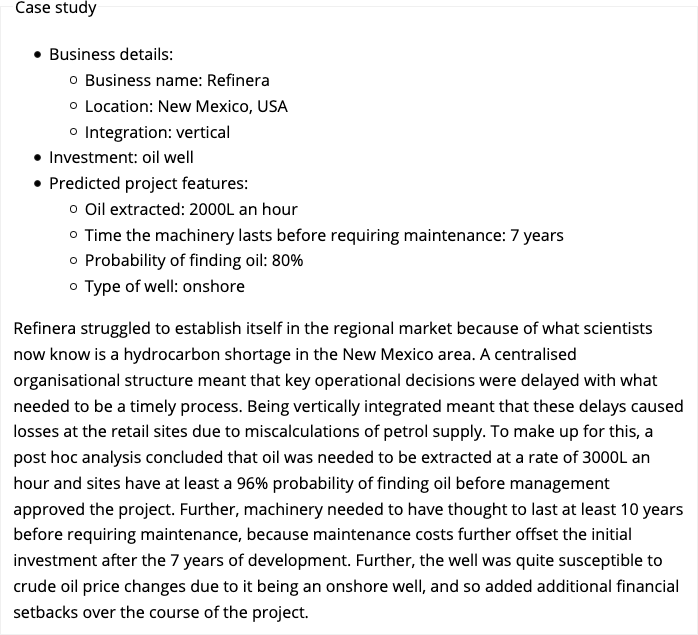
\includegraphics[width=1\linewidth]{anecdotal-bias-in-allocation-decisions_files/figure-latex/anecdote-similarity-high-1-1} \caption{Anecdote for participants in the high similarity condition in Experiment~1.}\label{fig:anecdote-similarity-high-1}
\end{figure}



\begin{figure}
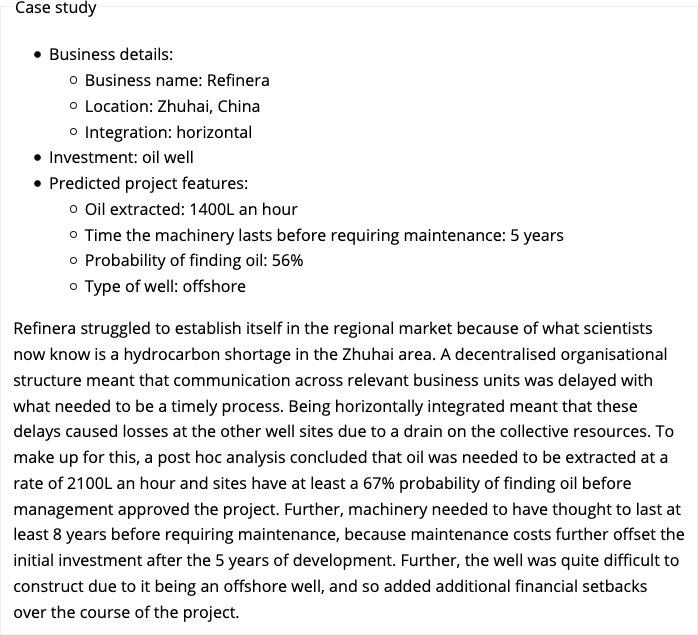
\includegraphics[width=1\linewidth]{anecdotal-bias-in-allocation-decisions_files/figure-latex/anecdote-similarity-low-1-1} \caption{Anecdote for participants in the low similarity condition in Experiment~1.}\label{fig:anecdote-similarity-low-1}
\end{figure}

\hypertarget{follow-up-questions}{%
\paragraph{Follow-up Questions}\label{follow-up-questions}}

Participants who were shown the anecdote were subsequently presented with
follow-up questions. They were asked about how similar they believed the
anecdote was to the target project, how relevant it was to their allocations and
how relevant it would be for their judgements about other projects of that type
(see Appendix~\ref{follow-up-materials-1}).

\hypertarget{procedure}{%
\subsubsection{Procedure}\label{procedure}}

Participants were introduced to the study through the general instructions
followed by the specific instructions for their condition. Participants were
then presented with the allocation task and a description of the focal projects.
All participants except those in the statistics only condition were also
presented with the anecdote description and analysis, and the follow-up
questions.

\hypertarget{results-anecdotes-1}{%
\subsection{Results}\label{results-anecdotes-1}}

\hypertarget{the-effect-of-similarity-on-anecdotal-bias}{%
\subsubsection{The Effect of Similarity on Anecdotal Bias}\label{the-effect-of-similarity-on-anecdotal-bias}}

Anecdotal bias was tested by comparing the statistics only condition with both
the high- and low-similarity anecdote \& statistics conditions (see
Figure~\ref{fig:plot-1-allocation-combined}). The omnibus one-way
ANOVA of these three conditions was significant,
\(F(2, 118) = 4.19\), \(p = .018\), \(\hat{\eta}^2_p = .066\).
Evidence of anecdotal bias is seen when participants allocate more to the
statistics only condition than to the anecdote \& statistics condition. Finding
this effect implies that the anecdote influenced participants to reduce their
allocation because the anecdote was unsuccessful. Planned comparisons show that
participants in the statistics only condition allocated more to the target
project compared with participants in the high-similarity anecdote \& statistics
condition,
\(\Delta M = -12.31\), 95\% CI \([-21.53, -3.09]\), \(t(118) = -2.64\), \(p = .009\); but not
the low-similarity anecdote with statistics condition,
\(\Delta M = -1.48\), 95\% CI \([-10.75, 7.80]\), \(t(118) = -0.31\), \(p = .753\). These findings
provide evidence of anecdotal bias in the high similarity condition only.



\begin{figure}
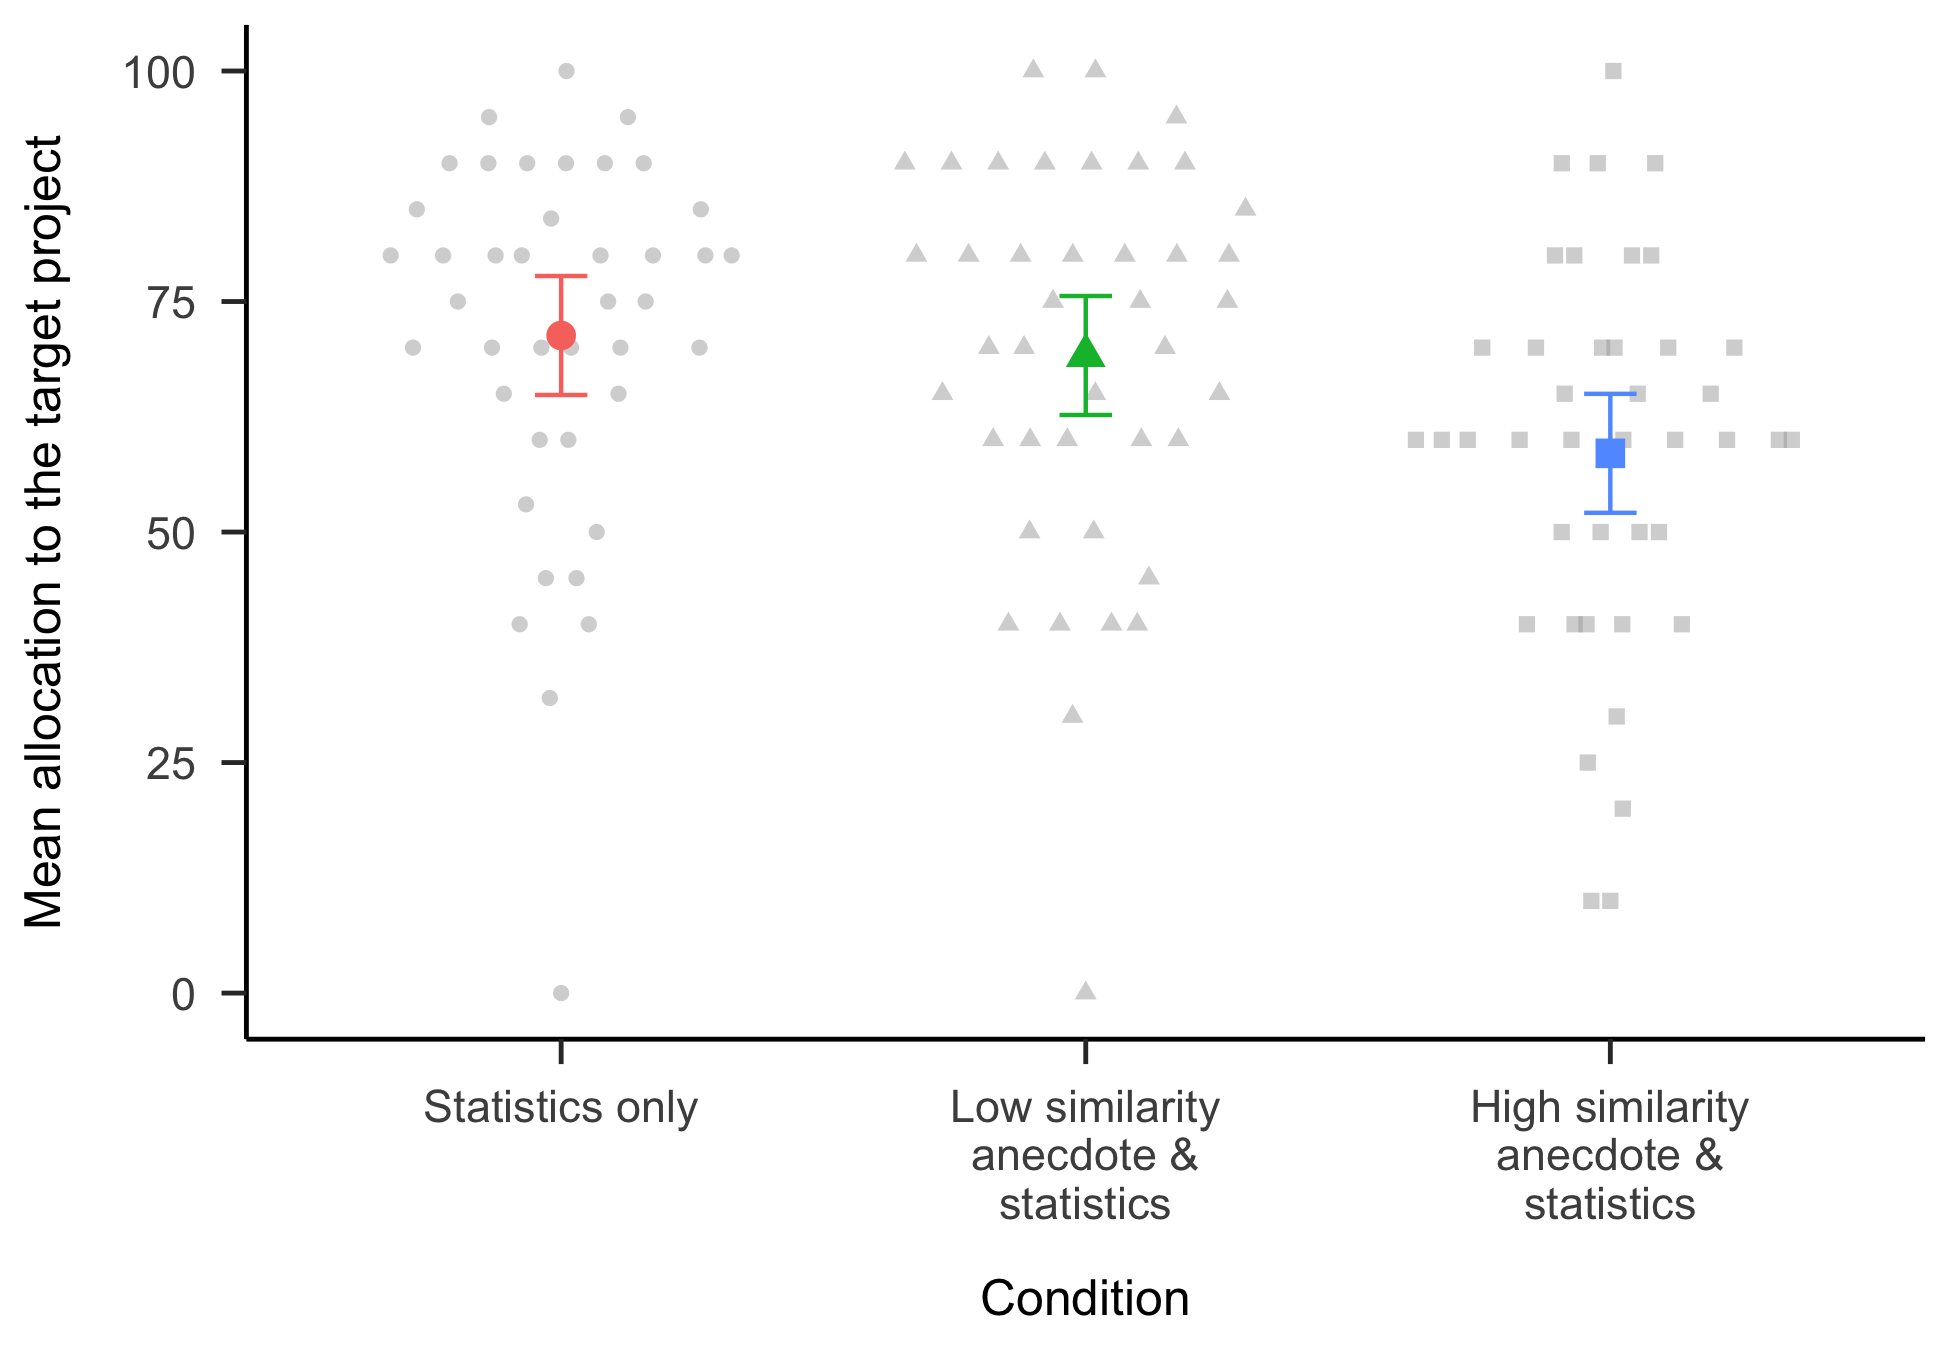
\includegraphics[width=1\linewidth]{anecdotal-bias-in-allocation-decisions_files/figure-latex/plot-1-allocation-combined-1} \caption{Mean allocation to the target project for the statistics only condition and the two anecdote \& statistics conditions. Error bars represent 95\% confidence intervals. Raw data are plotted in the background.}\label{fig:plot-1-allocation-combined}
\end{figure}

\hypertarget{the-effect-of-enhanced-statistics}{%
\subsubsection{The Effect of Enhanced Statistics}\label{the-effect-of-enhanced-statistics}}

In the enhanced statistics condition, we add an explanation of scientific
thinking to hint that aggregated data is likely to be more reliable than
anecdotes. The effect of enhanced statistics was investigated by testing the
interaction of anecdote similarity and evidence type (anecdote \& statistics and
anecdote \& enhanced statistics conditions, excluding the anecdote only and
statistics only conditions). As shown in
Figure~\ref{fig:plot-1-allocation}, the two-way interaction was not
significant, \(\Delta M = 3.89\), 95\% CI \([-8.86, 16.65]\), \(t(238) = 0.60\), \(p = .548\). Further, the
difference between the anecdote \& statistics condition and the anecdote \&
enhanced statistics condition (averaged over similarity conditions) was also not
significant, \(\Delta M = -0.12\), 95\% CI \([-6.50, 6.26]\), \(t(238) = -0.04\), \(p = .971\). This suggests that
providing participants with information about how to think statistically is not
sufficient to facilitate a focus on statistics.



\begin{figure}
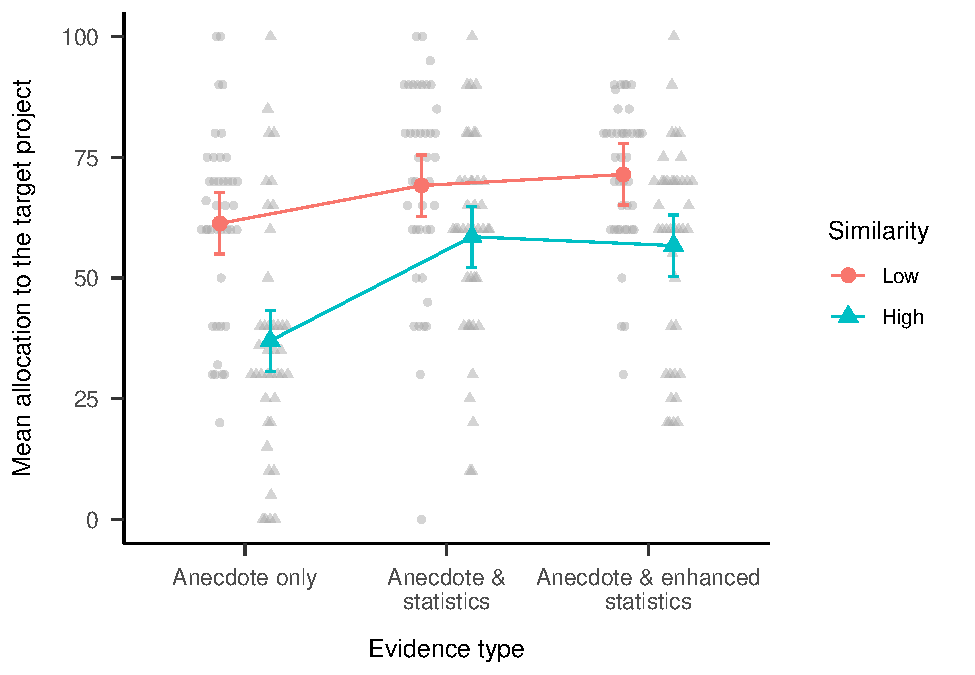
\includegraphics[width=1\linewidth]{anecdotal-bias-in-allocation-decisions_files/figure-latex/plot-1-allocation-1} \caption{Mean allocation to the target project, by anecdote similarity and evidence type conditions (excluding the statistics only condition). Error bars represent 95\% confidence intervals. Raw data are plotted in the background.}\label{fig:plot-1-allocation}
\end{figure}

\hypertarget{the-effect-of-statistics}{%
\subsubsection{The Effect of Statistics}\label{the-effect-of-statistics}}

To identify the influence of statistics on participants' allocations we compared
the anecdotes only condition to the high similarity anecdote \& statistics
condition (see Figure~\ref{fig:plot-1-allocation}). This tests
whether seeing the anecdote made participants disregard the statistics or
whether the statistics still influenced their decisions. We found that
participants allocated more in the high similarity anecdote \& statistics
condition compared with the anecdote only condition,
\(\Delta M = -21.56\), \(95\%\ \mathrm{CI}_\mathrm{\scriptsize Tukey(3)}\) \([-32.33, -10.80]\), \(t(238) = -4.72\), \(p_\mathrm{\scriptsize Tukey(3)} < .001\). This provides evidence of partial
anecdotal bias because the anecdote \& statistics condition was both lower than
the statistics only condition (shown above) and higher than the anecdote only
condition.

\hypertarget{relevance-ratings}{%
\subsubsection{Relevance Ratings}\label{relevance-ratings}}

Regression analyses were conducted to determine the relationship between
allocations and the follow-up relevance ratings. As shown in
Figure~\ref{fig:plot-1-lm-allocation-relevance-specific-alignment},
the specific relevance ratings interacted with similarity condition,
\(b = -2.84\), 95\% CI \([-4.80, -0.87]\), \(t(240) = -2.85\), \(p = .005\). It appears that
specific relevance ratings were related to allocations, but only in the high
similarity condition. That is, those in the high similarity condition allocated
less to the target project the more relevant they considered the negative
anecdote. Furthermore, there were no significant associations with the general
relevance ratings. This suggests that participants applied reasoning to the
connection between the anecdote and the target project as opposed to simply
reacting to the failed project and associating that with that project's
industry.



\begin{figure}
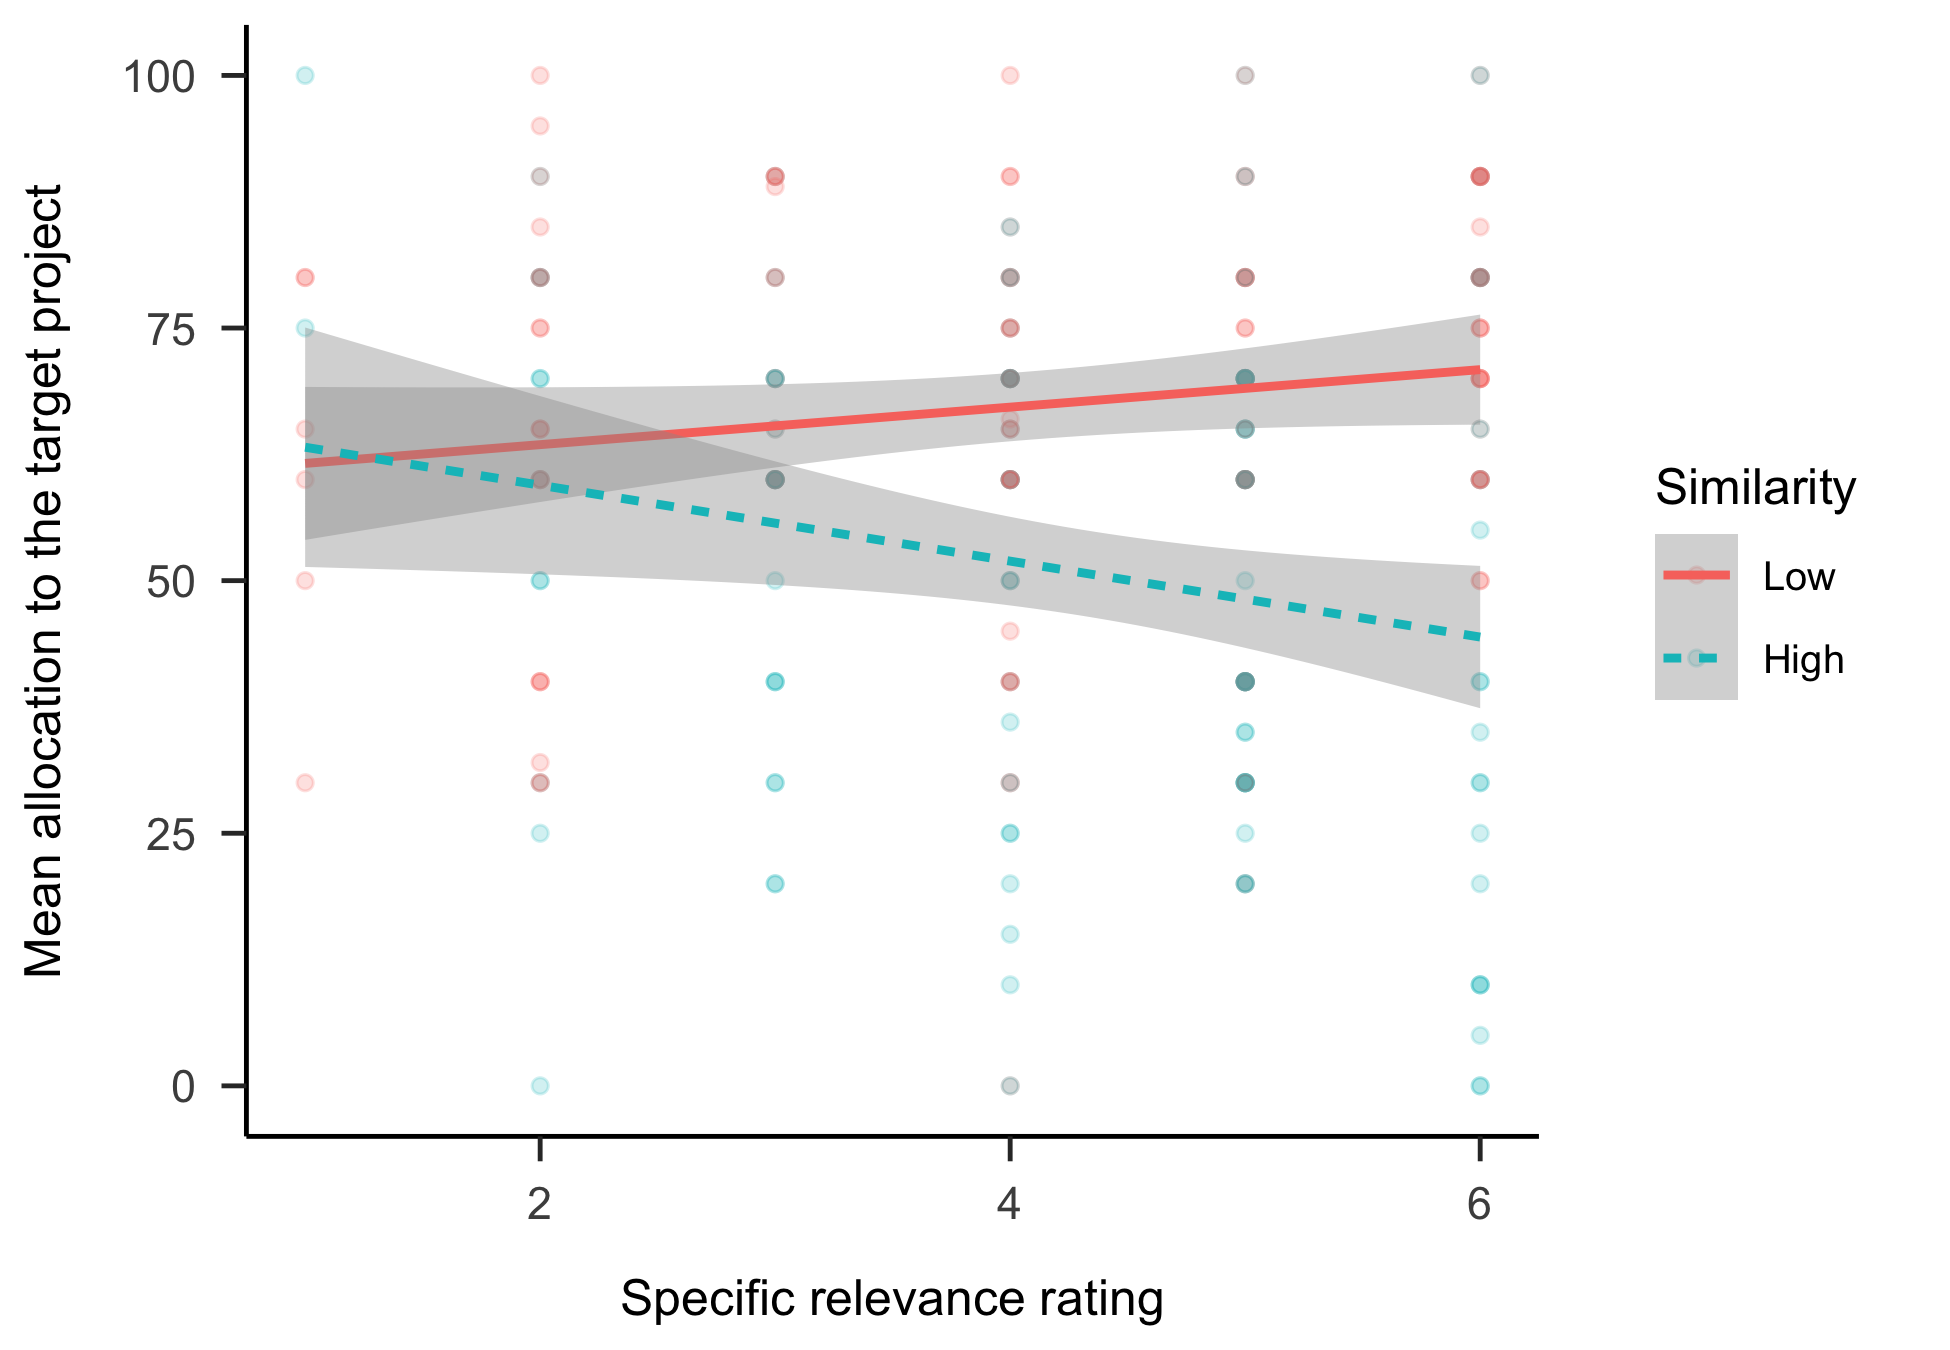
\includegraphics[width=1\linewidth]{anecdotal-bias-in-allocation-decisions_files/figure-latex/plot-1-lm-allocation-relevance-specific-alignment-1} \caption{Mean allocation to the target project, by specific relevance rating and similarity condition. LOESS method was used for smoothing over trials and the shading represents 95\% confidence intervals. Raw data are plotted in the background.}\label{fig:plot-1-lm-allocation-relevance-specific-alignment}
\end{figure}

\hypertarget{discussion}{%
\subsection{Discussion}\label{discussion}}

Hypothesis~\ref{hyp:anecdote-similarity-anecdotes-1} was supported.
Participants in the anecdote \& statistics condition allocated less capital to
the target project compared with those in the statistics only condition.
However, the novel finding was that this effect depended on anecdote similarity
because this only occurred in the high similarity condition, not in the low
similarity condition. Thus, while anecdotal bias was evident when the anecdote
was similar to the target project, participants were not influenced when the
causal mechanisms did not align. Congruent with
Hypothesis~\ref{hyp:statistics-anecdotes-1}, despite being influenced by the
anecdote, participants still made some use of the statistics. This is similar to
and replicates the finding of Wainberg et al. (\protect\hyperlink{ref-wainberg2013}{2013}).
Hypothesis~\ref{hyp:enhanced-statistics-anecdotes-1} was also not supported
because the added enhanced statistical instructions used to encourage
participants to use the statistical information did not reduce participants'
reliance on anecdotes. It is important to identify ways of reducing anecdote use
for situations in which it is inappropriate to use them. A promising simple
method to do so is to tell participants that ``small samples of observations tend
to have a higher probability of error while larger samples tend to be more
accurate'', which is part of what participants in the enhanced statistics
condition saw. Unfortunately, such simple instructions did not appear to work.

Experiment~1 was limited because it only considered a \emph{negative} anecdote; that
is, a failed project. In real life, however, case studies often have a
\emph{positive} valence; that is, the story of a successful company. In fact, in
business, it is possible that the anecdotes used are more likely to be positive
because of survivorship bias. Jaramillo et al. (\protect\hyperlink{ref-jaramillo2019}{2019}) found an anecdotal bias effect for
negative but not positive anecdotes. This may be because the study concerned
medical decisions and, in this domain being healthy may be the assumed default,
and so there is more room to lose than gain. In Experiment~2 (discussed in the
subsequent section) a positive anecdote was added to investigate whether
anecdote valence would affect anecdotal bias. In business, possible gains and
losses are both salient.

Important to the normative use of anecdotes is its relative similarity to a
target problem compared to the distribution of cases of which the anecdote is
sampled. It is unclear whether the effects found in Experiment~1 were related to
participants' perceptions of the type of sampling used to select the anecdotes.
The instructions in Experiment~1 did not explain how the anecdote displayed to
participants was chosen. Whether sampling is believed to be intentional or
random has been shown to affect people's induction and decision-making (e.g., \protect\hyperlink{ref-hayes2019}{Hayes et al., 2019}). Further, Kahneman and Tversky (\protect\hyperlink{ref-kahneman1982}{1982}) suggest that people are likely
to be insensitive to distributional information. In the present experiments,
participants' sampling assumptions may have changed the extent to which they
used the anecdote in their decisions. For example, it may be rational to choose
the anecdote over the aggregated data if (a) the anecdote was not sampled
randomly from a pool of anecdotes, and (b) the anecdote had a greater similarity
to the target project compared with other anecdotes in the pool in relevant
ways. That is, if the anecdote were chosen because of its high relevance to the
target project, it would be irrational to ignore it. In Experiment~1, it was
unclear whether participants may have held these beliefs. To control for these
assumptions, in Experiment~2, the instructions further clarified that the
anecdote (a) was sampled randomly from a pool of anecdotes, and (b) was not
significantly more similar to the target project than any of the other anecdotes
in the pool.

\hypertarget{anecdotes-2}{%
\section{Experiment~2}\label{anecdotes-2}}

The novel finding in Experiment~1 was that the anecdotal bias effect depends on
anecdote similarity. That is, participants allocated less capital to a project
when presented with an anecdote and conflicting statistics compared with when
they were presented with the statistics only. However, this effect was stronger
when the anecdote was similar to the current task compared with when it was less
similar. A negative anecdote only was used Experiment~1 because previous
research has found anecdotal bias for negative but not for positive anecdotes
(\protect\hyperlink{ref-jaramillo2019}{Jaramillo et al., 2019}). However, Jaramillo et al. (\protect\hyperlink{ref-jaramillo2019}{2019}) investigated medical decision-making,
and the effect of anecdote valence, which may be different in a less salient
business context. In the study by Jaramillo et al. (\protect\hyperlink{ref-jaramillo2019}{2019}), the positive anecdote involved
a treatment that led to a reduction in symptoms, while the negative anecdote
involved symptoms persisting. This framing may have led participants to perceive
the positive anecdote as a return to a reference point and the negative anecdote
as a continuation of a reduction in wellbeing relative to the reference point.
In business, however, both successful and failed business projects represent a
deviation from a reference point. To test this difference further, manipulation
of anecdote valence was added to Experiment~2.

To increase the experiment's power, anecdote valence and anecdote similarity
were manipulated within subjects. Further, Experiment~2 did not include the
anecdote \& enhanced statistics condition because Experiment~1 found no
evidence for its effect. All participants saw the statistics only condition,
which did not contain an anecdote; therefore, this did not need to be
manipulated between subjects. Therefore, each participant was shown five
displays: one for the statistics only condition, and four for either the
anecdote only condition or the anecdote \& statistics condition. These four
anecdote displays consisted of the similarity (low and high) \(\times\) valence
(negative and positive) conditions.

In Experiment~1, assumptions about the pool from which the anecdote was sampled
were not clarified. In Experiment~2, participants were told that the anecdote
was sampled randomly and that it was not uniquely similar to the target project.
This was expected to lead to a reliance on statistical evidence, regardless of
the anecdote's similarity. However, people often struggle to use statistical
concepts presented descriptively, as seen in the enhanced statistics condition
in Experiment~1. Therefore, it was expected that the results of Experiment~1
would be replicated for the negative valence condition. Further, it was expected
that there would be a reverse effect in the positive valence condition.
Appendix~\ref{hypothesised-effects-anecdotes-2} shows a simulation of the
hypothesised effects.

The main effect of interest is the effect of anecdote similarity on anecdotal
bias. However, because in Experiment~2 all participants were presented with the
statistics only condition, a difference score was calculated to simplify the
analyses. Specifically, this was the difference between the allocation in the
anecdote \& statistics conditions and the relevant allocation in the statistics
only condition. A score that is different from zero indicates deviation from the
allocation when only statistics were shown. The values in the anecdote
descriptions were different for the positive anecdotes than for the negative
anecdotes. However, the statistics only condition was the same for both.
Therefore, the difference scores for the positive anecdotes had to be
transformed further to directly compare the magnitude of the difference from the
statistics only condition between the positive and negative anecdote
(respectively). We did this by multiplying the positive anecdote difference
score by \(-1\). This means that the bigger the difference score, the bigger the
anecdotal effect for both valence conditions. Therefore, Experiment~2 tested the
following hypotheses:

\begin{hypothesis}[anecdotal bias difference score]
\protect\hypertarget{hyp:anecdote-similarity-2}{}\label{hyp:anecdote-similarity-2}The difference between budget allocations to the target project in the
statistics only condition and the anecdote \& statistics condition will be higher
when the anecdote is similar to the target project compared with when it is
less similar.
\end{hypothesis}

Jaramillo et al. (\protect\hyperlink{ref-jaramillo2019}{2019}) found that the effect of a negative medical anecdote was stronger
compared with a positive one. However, business is dissimilar from medicine
because both gains and losses are more salient in medicine than business.
Therefore, Experiment 2 tested the following hypothesis:

\begin{hypothesis}[anecdotal bias difference score valence interaction]
\protect\hypertarget{hyp:anecdote-similarity-valence-interaction-2}{}\label{hyp:anecdote-similarity-valence-interaction-2}The effect of similarity on the anecdotal bias difference score will not depend
on anecdote valence.
\end{hypothesis}

Similar to both Wainberg et al. (\protect\hyperlink{ref-wainberg2013}{2013}) and Hypothesis~\ref{hyp:statistics-anecdotes-1},
Experiment~1 found that participants do integrate statistics in their decisions
to some extent. This effect was expected to be replicated in Experiment~2.
Therefore, Experiment~2 tested the following hypothesis:

\begin{hypothesis}[effect of statistics]
\protect\hypertarget{hyp:statistics-anecdotes-2}{}\label{hyp:statistics-anecdotes-2}Budget allocations to the target project will be higher
for the high-similarity anecdote \& statistics condition than for the
high-similarity anecdote only condition.
\end{hypothesis}

\begin{hypothesis}[effect of statistics valence interaction]
\protect\hypertarget{hyp:statistics-valence-interaction-2}{}\label{hyp:statistics-valence-interaction-2}The effect of statistics will not depend on anecdote valence.
\end{hypothesis}

\hypertarget{method}{%
\subsection{Method}\label{method}}

\hypertarget{participants-1}{%
\subsubsection{Participants}\label{participants-1}}

Ninety-six participants (50 female) were recruited from the online recruitment platform Prolific. Participants were compensated at a rate of \pounds 5 an hour (Prolific is based in the UK). The average age was 41.69 years (\emph{SD} = 11.29, \emph{min.} = 27, \emph{max.} = 74). Participants reported an average of 7.19 years (\emph{SD} = 8.34, \emph{min.} = 0, \emph{max.} = 43) working in a business setting, and an average of 3.91 years (\emph{SD} = 7.67, \emph{min.} = 0, \emph{max.} = 50) of business education. The mean completion time of the task was 14.98 min.~Table~\ref{tab:condition-allocation-2}
shows the allocation of participants to the different conditions. Anecdote
similarity and valence were manipulated within subjects. Therefore, each
participant was assigned to one of two between-subjects evidence type conditions
(anecdote only and anecdote \& statistics) and saw five displays (statistics
only, and one of each of the four similarity and valence conditions).
Appendix~\ref{power-analysis-2} describes the power analysis
conducted to arrive at this sample size.

\begin{table}[tbp]

\begin{center}
\begin{threeparttable}

\caption{\label{tab:condition-allocation-2}Experiment 2 group allocation.}

\begin{tabular}{ll}
\toprule
Evidence type & \multicolumn{1}{c}{N}\\
\midrule
Anecdote \& statistics & 48\\
Anecdote only & 48\\
Total & 96\\
\bottomrule
\end{tabular}

\end{threeparttable}
\end{center}

\end{table}

\hypertarget{materials}{%
\subsubsection{Materials}\label{materials}}

\hypertarget{instructions}{%
\paragraph{Instructions}\label{instructions}}

Participants were shown similar instructions to those in Experiment~1. The
general instructions page included a test of the basic information expressed in
the instructions. This test also functioned as an attention check. As in
Experiment~1, participants were also shown instructions that were specific to
their condition. These were shown on the same page as the rest of the project
display, above the case study and focal projects. The instructions clarified
that the anecdote had been randomly sampled and that all anecdotes in the pool
were equally similar to the target project.
Appendix~\ref{instructions-materials-2-appendix} shows the
instructions used in Experiment~2.

\hypertarget{allocation-2}{%
\paragraph{Allocation Task}\label{allocation-2}}

As in Experiment~1, the allocation task included a table describing the two
focal projects and (apart from the statistics only condition) a description and
analysis of an anecdote.
Figures~\ref{fig:allocation-anecdote-valence-negative-similarity-low-2}
and~\ref{fig:allocation-target-valence-negative-similarity-low-2}
show the anecdote and focal projects, respectively, for the negative valence,
low similarity condition.
Figures~\ref{fig:allocation-anecdote-valence-positive-similarity-high-2}
and~\ref{fig:allocation-target-valence-positive-similarity-high-2}
show the anecdote and focal projects, respectively, for the positive valence,
high similarity conditions. In the statistics only condition, participants were
only shown the focal projects display.

The following were counterbalanced: (a) project variation (five latin square
variations), which is the association of each display content with each
within-subject condition; and (b) anecdote variation (two variations), which is
the association of each project display and being either the target or
comparison project. Table column order and project display order were
randomised.



\begin{figure}

\includegraphics[width=1\linewidth]{anecdotal-bias-in-allocation-decisions_files/figure-latex/allocation-anecdote-valence-negative-similarity-low-2-1} \caption{An example of the anecdote display in the negative valence, low similarity condition of Experiment~2.}\label{fig:allocation-anecdote-valence-negative-similarity-low-2}
\end{figure}



\begin{figure}
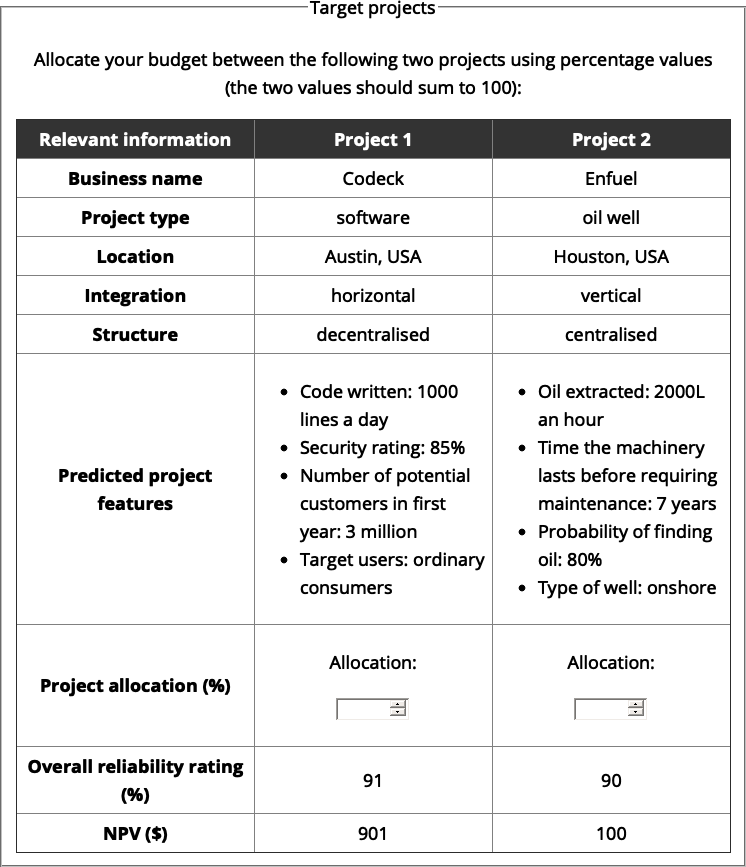
\includegraphics[width=1\linewidth]{anecdotal-bias-in-allocation-decisions_files/figure-latex/allocation-target-valence-negative-similarity-low-2-1} \caption{An example of the focal projects in the negative valence, low similarity condition of Experiment~2. Here, Project~1 was the target project and Project~2 was the comparison project.}\label{fig:allocation-target-valence-negative-similarity-low-2}
\end{figure}



\begin{figure}

\includegraphics[width=1\linewidth]{anecdotal-bias-in-allocation-decisions_files/figure-latex/allocation-anecdote-valence-positive-similarity-high-2-1} \caption{An example of an anecdote display in the positive valence, high similarity condition of Experiment~2.}\label{fig:allocation-anecdote-valence-positive-similarity-high-2}
\end{figure}



\begin{figure}
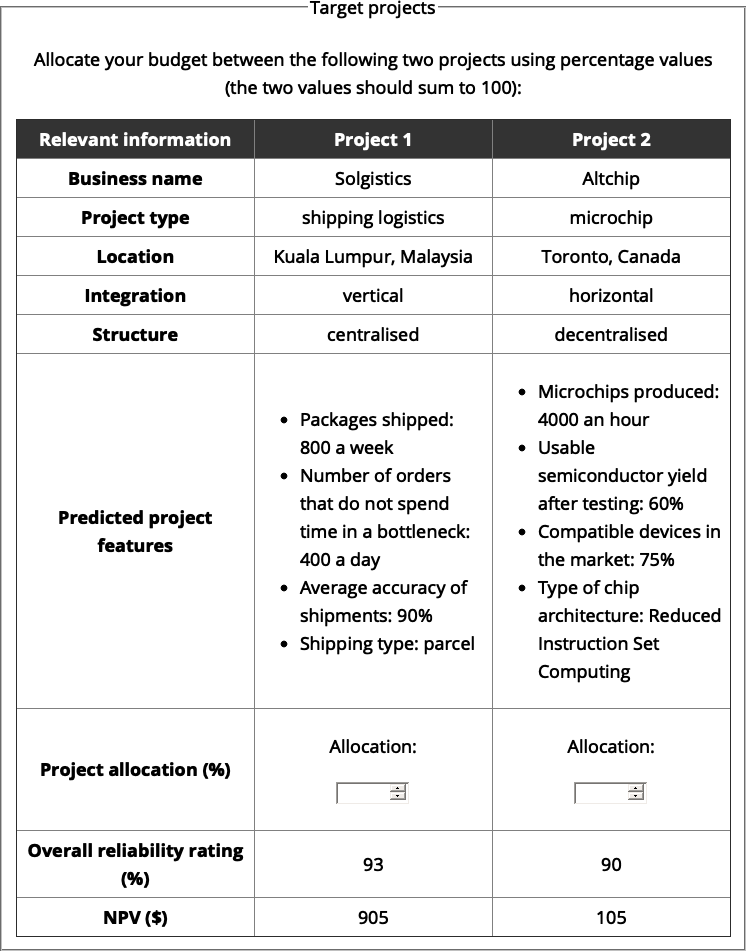
\includegraphics[width=1\linewidth]{anecdotal-bias-in-allocation-decisions_files/figure-latex/allocation-target-valence-positive-similarity-high-2-1} \caption{An example of the focal projects in the positive valence, high similarity condition of Experiment~2. Here, Project~2 was the target project and Project~1 was the comparison project.}\label{fig:allocation-target-valence-positive-similarity-high-2}
\end{figure}

\hypertarget{interstitial-page}{%
\paragraph{Interstitial Page}\label{interstitial-page}}

Prior to the display, participants were shown an interstitial page, which was
used to (a) introduce the display and (b) check the participant's attention
(given that no input was required, participants could easily skip the page
without reading the text). See
Appendix~\ref{interstitial-materials-2}.

\hypertarget{follow-up-questions-1}{%
\paragraph{Follow-up Questions}\label{follow-up-questions-1}}

Participants were shown similar follow-up questions as in Experiment~1, except
that in Experiment~2, rating scales were 1--7 instead of 1--6. See
Appendix~\ref{follow-up-materials-2} for a sample display of the
follow-up questions.

\hypertarget{procedure-1}{%
\subsubsection{Procedure}\label{procedure-1}}

Participants were introduced to the study via the general instructions page.
They were then shown five sets (presented in a random order) containing three
pages each: an interstitial page, a page showing the allocation task, and a page
with follow-up questions (except for the statistics only condition, in which
participants were not shown the follow-up questions page). The interstitial
pages introduced each display and checked participants' attention to the task.
Each allocation task page contained specific instructions relevant to the
condition followed by the anecdote analysis and description, and the description
of the two focal projects. The only exception was the statistics only display,
for which there was no anecdote description or analysis.

\hypertarget{results}{%
\subsection{Results}\label{results}}

This section reports only the data relevant to the Experiment~2 hypotheses. See
Appendix~\ref{results-2-appendix} for manipulation check analyses.

\hypertarget{anecdotal-bias-depends-on-anecdote-similarity}{%
\subsubsection{Anecdotal Bias Depends on Anecdote Similarity}\label{anecdotal-bias-depends-on-anecdote-similarity}}

To investigate whether anecdotal bias depended on anecdote similarity, the raw
budget allocation values were transformed to create a dependant value that both
expressed the magnitude of anecdotal bias and allowed equivalent comparison
across valence conditions. To quantify the magnitude of anecdotal bias we
calculated a difference score between allocations in the statistics only
condition and the two anecdote \& statistics conditions (high and low
similarity). During the experiment all participants saw a statistics only
condition in which the target project statistics were higher than those in the
comparison project. However, this was only equivalent to what participants saw
in the negative valence condition. Therefore, for the positive valence condition
we calculated a difference score using the inverse value of the allocation in
the statistics only condition---its difference from 100. Subsequently, the
difference scores in the positive valence condition were multiplied by -1 to
make the comparison between valence conditions equivalent. This means that a
higher value indicates a stronger effect of similarity on the magnitude of
anecdotal bias.

As shown in Figure~\ref{fig:plot-2-allocation-difference}, the main
effect of similarity was significant and very large (\protect\hyperlink{ref-cohen1988}{Cohen, 1988}),
\(F(1, 47) = 30.66\), \(p < .001\), \(\hat{\eta}^2_p = .395\). However, the similarity \(\times\)
valence interaction was not significant,
\(F(1, 47) = 0.53\), \(p = .469\), \(\hat{\eta}^2_p = .011\), as was the main effect
of valence, \(F(1, 47) = 0.00\), \(p = .958\), \(\hat{\eta}^2_p = .000\). This provides evidence
that anecdotal bias depends on anecdote similarity for both negative and
positive anecdotes. Specifically, there was more influence of the anecdote when
it is similar than when it is less similar. Participants appeared to be
sensitive to the relevance of the anecdote to the target problem. However, the
magnitude of this effect did not differ between negative and positive anecdotes.

\newpage

\begin{landscape}



\begin{figure}
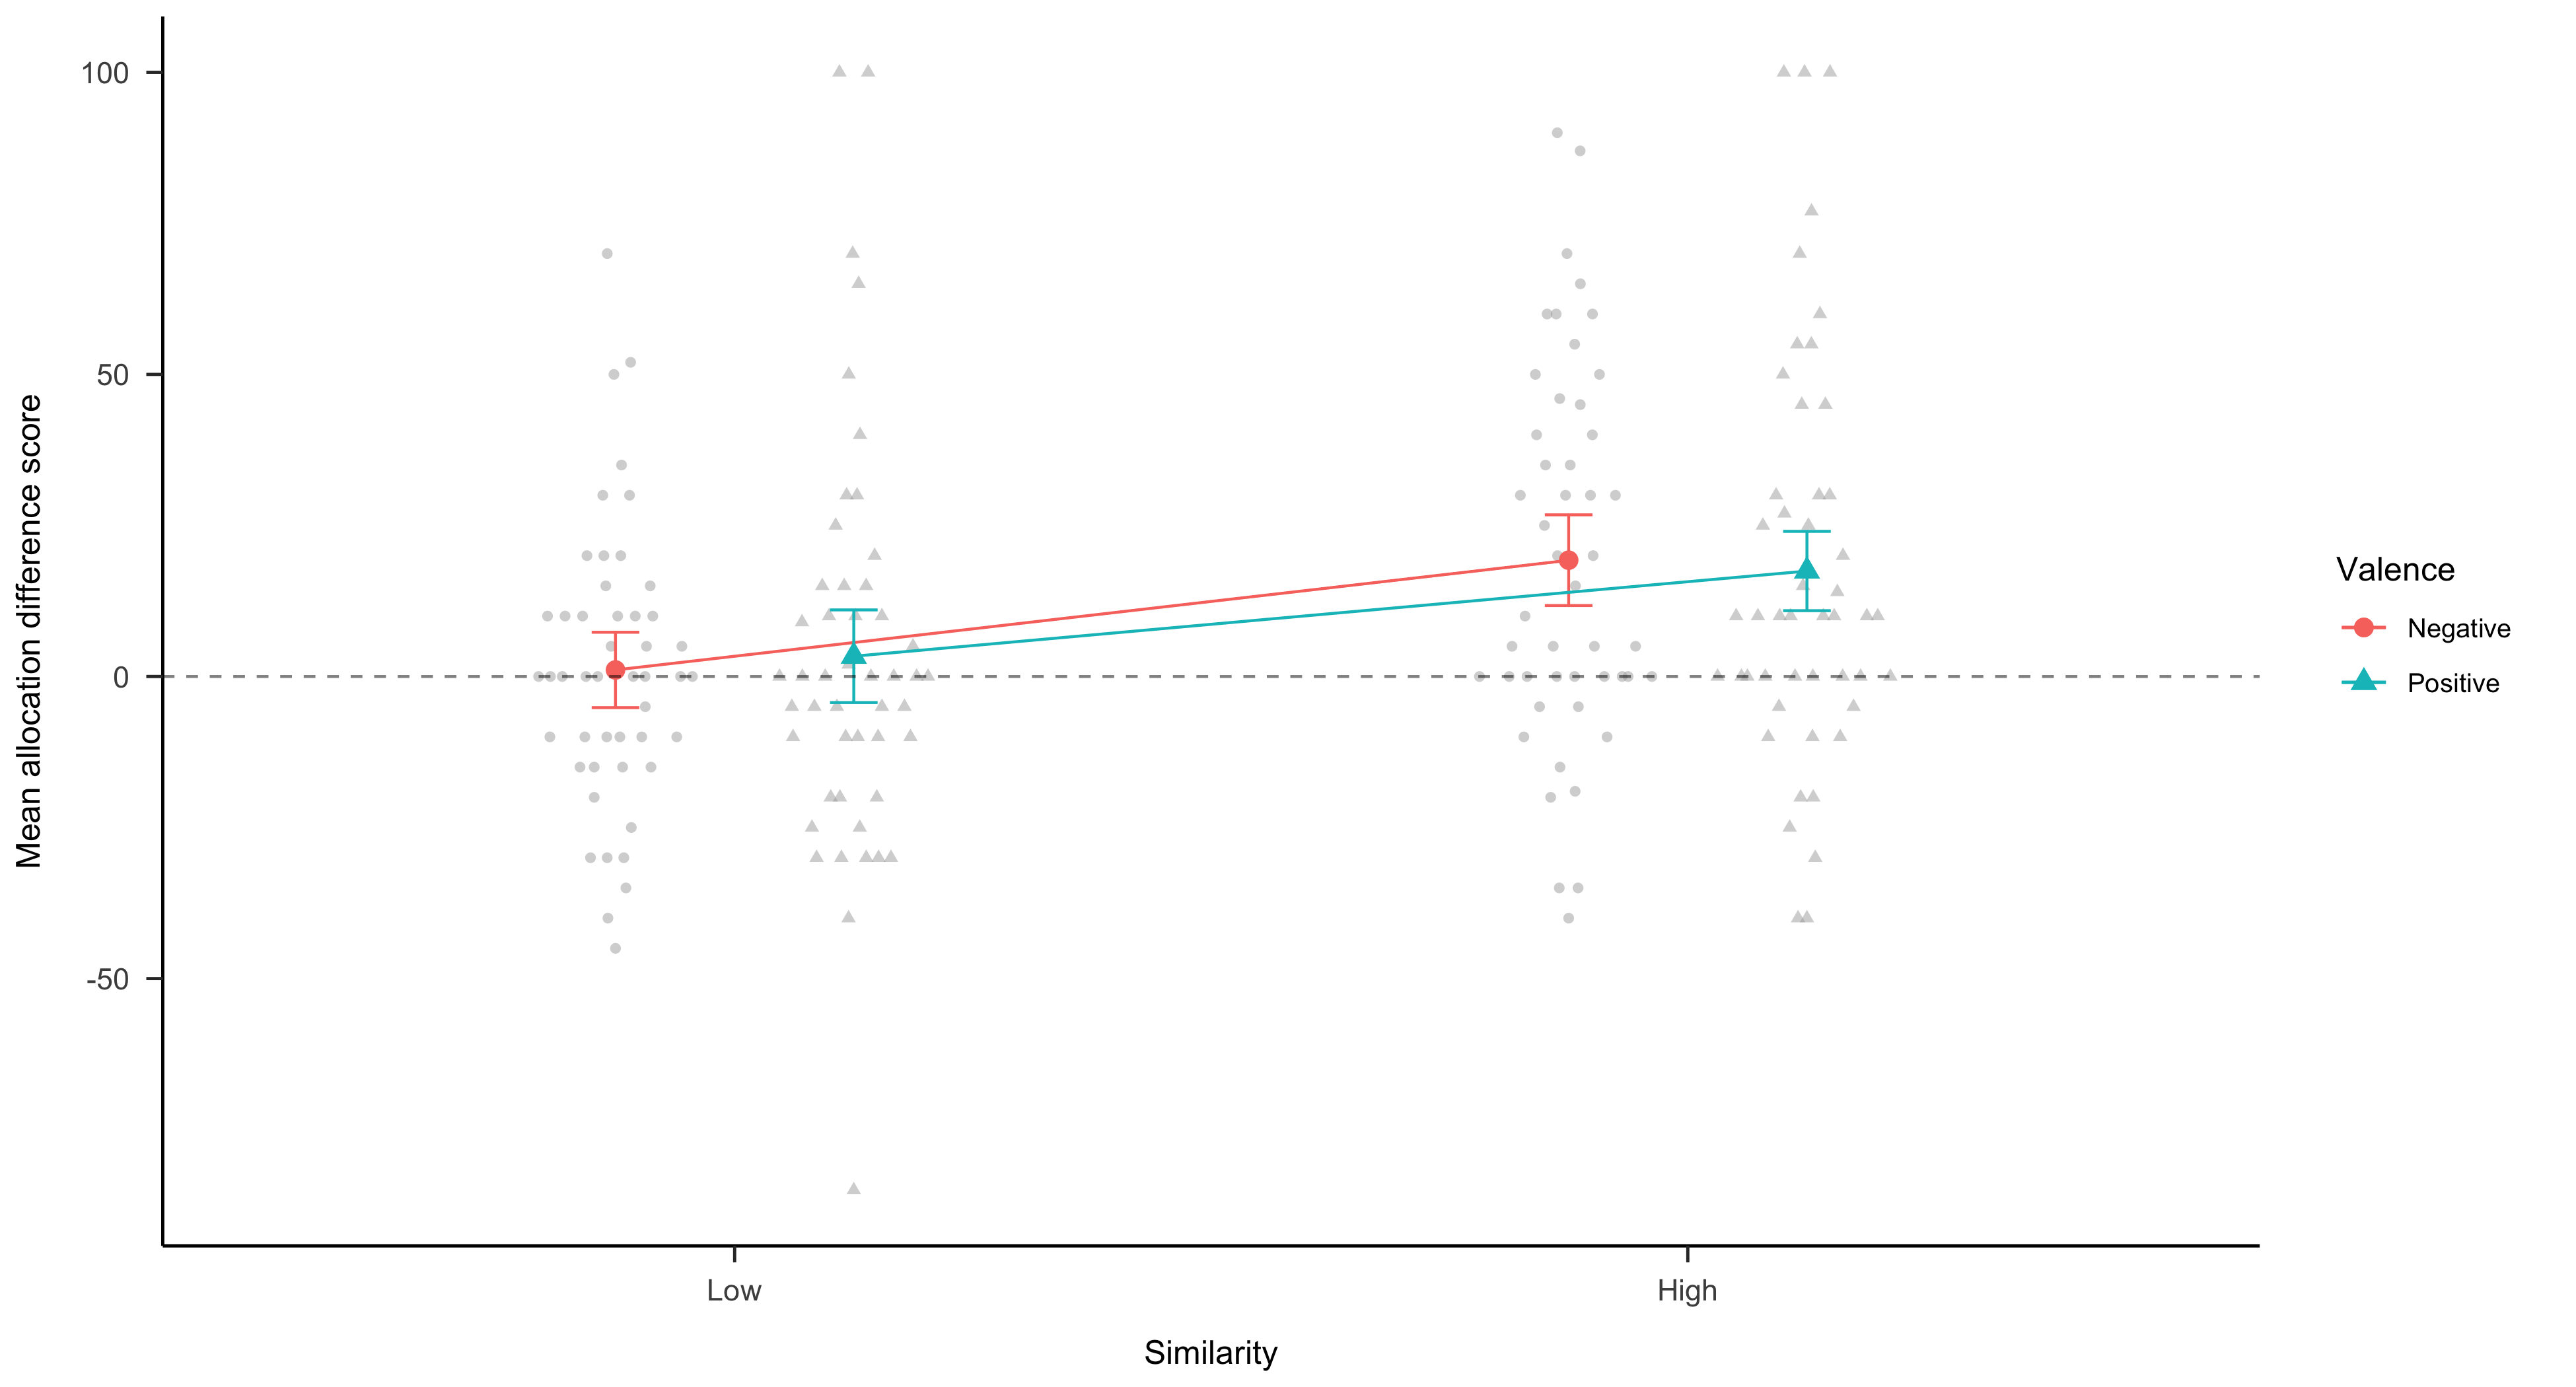
\includegraphics[width=1\linewidth]{anecdotal-bias-in-allocation-decisions_files/figure-latex/plot-2-allocation-difference-1} \caption{Mean transformed allocation difference between the statistics only condition and the anecdote \& statistics condition, by similarity and valence conditions. The positive valence allocations were transformed to create equivalent comparisons. Before creating the difference score, we calculated the difference of the statistics only allocation and 100 for positive valence. The positive valence difference score was then multiplied by -1. The horizontal dashed line indicates no effect of anecdote and values above this line show a stronger effect of the anecdote. Error bars represent 95\% confidence intervals, calculated from the within-subjects standard errors using the method from Cousineau and O'Brien (\protect\hyperlink{ref-cousineau2014}{2014}). Raw data are plotted in the background.}\label{fig:plot-2-allocation-difference}
\end{figure}

\end{landscape}

\newpage

\hypertarget{effect-of-statistics}{%
\subsubsection{Effect of Statistics}\label{effect-of-statistics}}

As in Experiment~1, Experiment~2 investigated the extent to which statistical
information influenced participants' allocations in the high similarity
condition. As shown in Figure~\ref{fig:plot-2-allocation}, only the
main effect of evidence type was significant in the high similarity condition,
\(F(1, 94) = 13.60\), \(p < .001\), \(\hat{\eta}^2_p = .126\). The main
effect of valence was not significant,
\(F(1, 94) = 0.00\), \(p = .956\), \(\hat{\eta}^2_p = .000\). as was the
interaction,
\(F(1, 94) = 0.24\), \(p = .626\), \(\hat{\eta}^2_p = .003\). This
provides evidence that participants' allocations were not solely influenced by
anecdotes but were also influenced by the aggregated data. This effect was
equivalent between negative and positive anecdotes.



\begin{figure}
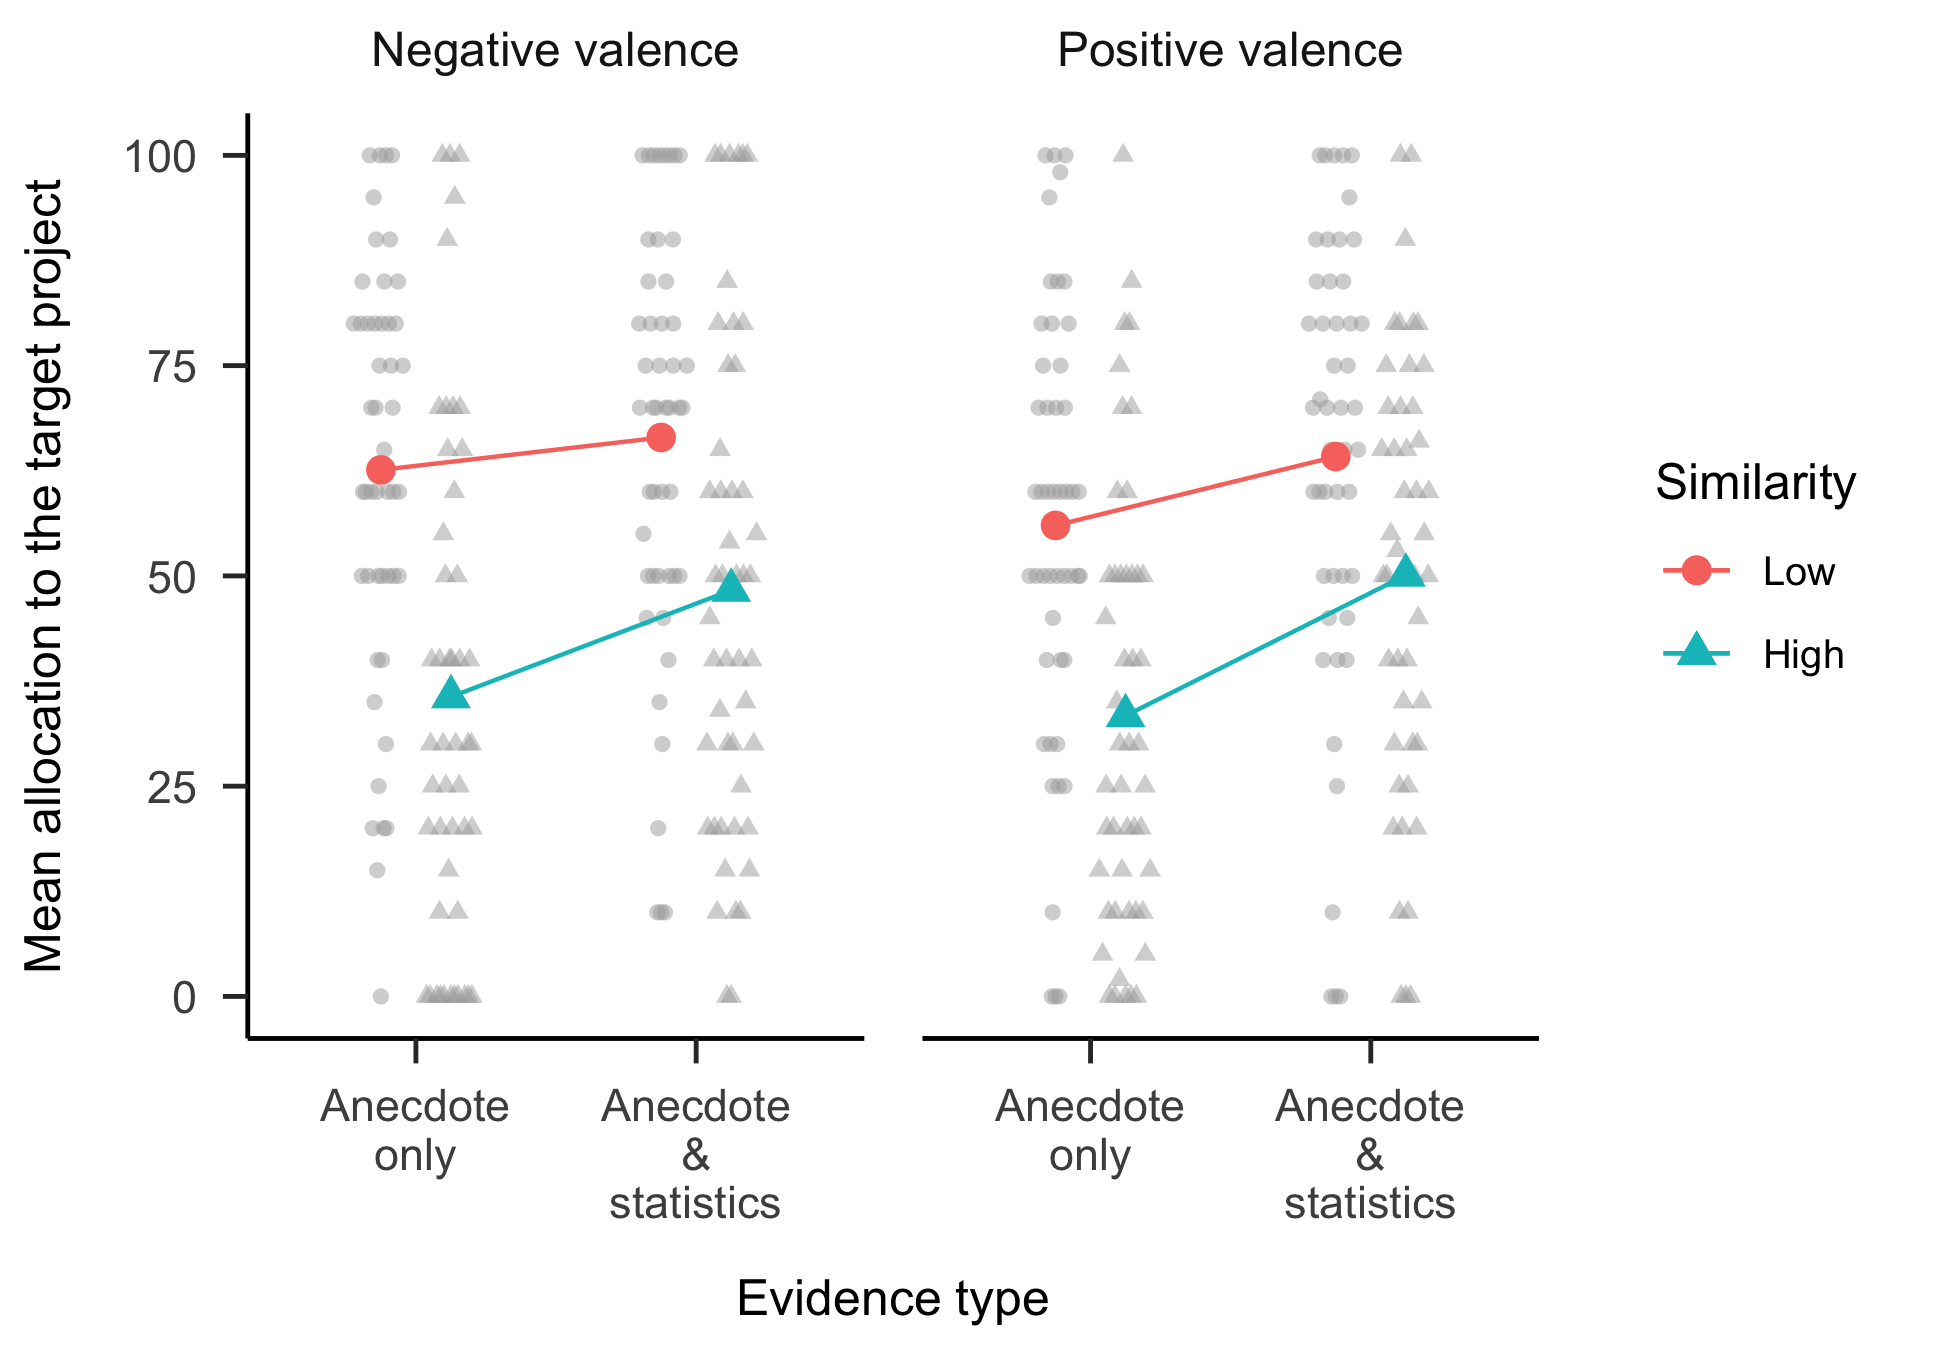
\includegraphics[width=1\linewidth]{anecdotal-bias-in-allocation-decisions_files/figure-latex/plot-2-allocation-1} \caption{Transformed mean allocation to the target project, by evidence type, similarity, and valence conditions. We calculated the difference of positive valence allocations from 100 to create equivalent comparisons. In mixed factorial designs, error bars cannot be used to make inferences by ``eye'' across all conditions. Therefore, error bars are not included. Raw data are plotted in the background.}\label{fig:plot-2-allocation}
\end{figure}

\hypertarget{relevance-ratings-1}{%
\subsubsection{Relevance Ratings}\label{relevance-ratings-1}}

Regression analyses were conducted to determine the relationship between
allocations and the follow-up relevance ratings.
Figure~\ref{fig:plot-2-lm-allocation-relevance-specific-similarity}
shows these data. In Experiment~1 we found that specific relevance ratings were
related to project allocations, but only in the high similarity rating. This
implied added evidence that participants were reasoning about the relevance of
the projects based on the provided details, rather than just based on a surface
association to the project type. In Experiment~2, while the specific relevance
ratings for negative anecdotes showed the same trends as in Experiment~1, the
interaction was not significant. Similarly, the ratings trends for positive
anecdotes were as hypothesised, but their interaction not significant. It
appears that specific relevance ratings were related to allocations, but only in
the high similarity condition. Further, there were no significant associations
with the general relevance ratings. This provides limited evidence that people
were explicitly reasoning about the connection between the anecdote and target.



\begin{figure}
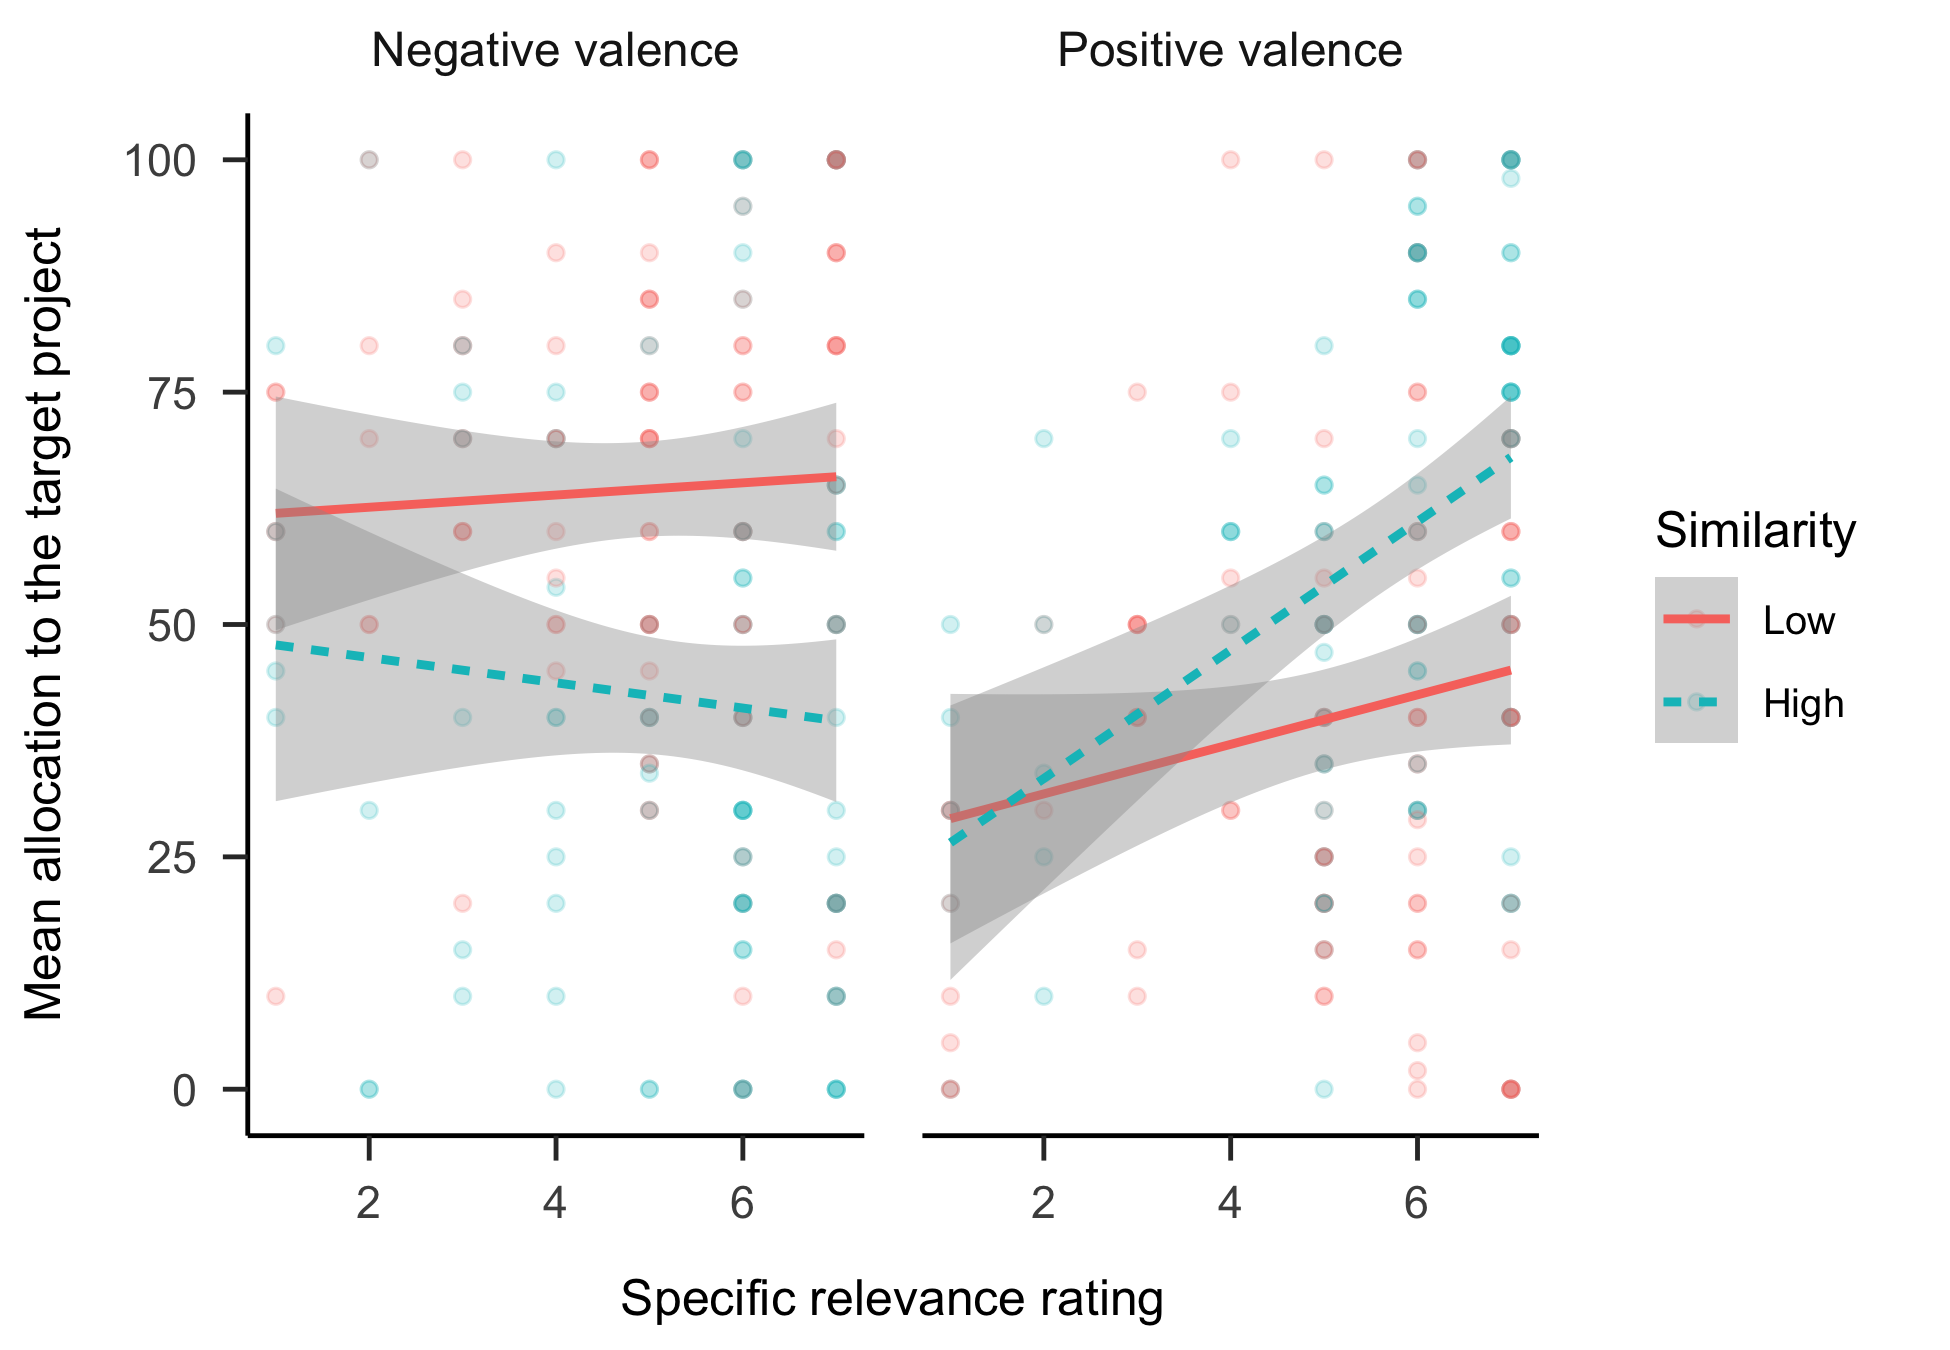
\includegraphics[width=1\linewidth]{anecdotal-bias-in-allocation-decisions_files/figure-latex/plot-2-lm-allocation-relevance-specific-similarity-1} \caption{Mean allocation to the target project, by specific relevance rating, similarity condition, and valence condition. LOESS method was used for smoothing over trials and the shading represents 95\% confidence intervals. Raw data are plotted in the background.}\label{fig:plot-2-lm-allocation-relevance-specific-similarity}
\end{figure}

\hypertarget{similarity-distribution-clarification}{%
\subsubsection{Similarity Distribution Clarification}\label{similarity-distribution-clarification}}

In Experiment~2, participants were told that each anecdote they were considering
was not significantly more similar to the target project than the other projects
in the aggregated data. This addition to the instructions was designed to rule
out the possibility that participants were assuming that the anecdote was unique
in its similarity to the target. We did not explicitly manipulate this variable
in a single experiment, but the anecdotal bias effect was no smaller in
Experiment~2 than in Experiment~1. To make an equivalent comparison we
considered the difference between the high similarity anecdote \& statistics
condition and the statistics only condition for negative anecdotes. In
Experiment~1, \(\hat{\eta}^2_p = .056\), whereas in
Experiment~2, \(\hat{\eta}^2_p = .277\).

\hypertarget{discussion-1}{%
\subsection{Discussion}\label{discussion-1}}

Hypothesis~\ref{hyp:anecdote-similarity-2} was supported because participants
showed a stronger anecdotal bias effect when anecdotes had greater similarity to
the target project and effect did not depend on valence. This was the same
finding as Experiment 1 despite the instructions making it clear that the
anecdote was not significantly more similar to the target project than the other
projects in the aggregated data. Further, as per
Hypothesis~\ref{hyp:statistics-anecdotes-2}, participants incorporated
statistical information in their judgements. As per
Hypotheses~\ref{hyp:anecdote-similarity-valence-interaction-2}
and~\ref{hyp:statistics-valence-interaction-2}, both the anecdotal bias effect
and effect of statistics did not depend on anecdote valence. Unlike in
Experiment~1, the relevance rating data did not provide as clear indication that
participants were using only the specific project information rather than merely
its industry.

Therefore, Experiment~2 found that participants use anecdote similarity in their
decisions but not information about the relative similarity of the anecdote to
the rest of the data. That is, participants seem to be considering only one
factor for optimal anecdote use but not the other. Further, unlike in the
medical domain, the effect of anecdotes in financial decision-making does not
depend on anecdote valence. The lack of asymmetry between valence conditions is
surprising given the effect of loss aversion on people's decisions
(\protect\hyperlink{ref-kahneman1979}{Kahneman \& Tversky, 1979}). This is discussed further in the General Discussion. Further,
similar to the findings of Experiment~1, and as in those of Wainberg et al. (\protect\hyperlink{ref-wainberg2013}{2013}), the
anecdotal bias effect does not appear to be complete, with statistics still
playing some role in participants' decisions, despite the effect of the
anecdote.

\hypertarget{general-discussion}{%
\section{General Discussion}\label{general-discussion}}

The present studies found that, in the capital allocation context, people's
decisions are influenced by anecdotes, even when aggregated data are available,
providing evidence for anecdotal bias (e.g., \protect\hyperlink{ref-wainberg2018}{Wainberg, 2018}). Further, we found
an effect of anecdote similarity, helping clarify the mixed findings on this
influence (e.g., \protect\hyperlink{ref-hoeken2009}{Hoeken \& Hustinx, 2009}). There were three novel findings that characterise
how anecdotes support inductive thinking: (a) the anecdotal bias effect was only
seen when participants considered the anecdote sufficiently similar to the
target project; (b) people did not consider descriptions of sample distribution
information, which could have helped to inform their decisions; and (c) these
effects were found with the same magnitude in both negative and positive
anecdotes. This is surprising since other work showed that generalisations are
sensitive to sampling (\protect\hyperlink{ref-carvalho2021}{Carvalho et al., 2021}). Normative use of anecdotes would consider
(a) the underlying structure relevant to what caused the key outcome in the
anecdote and whether it applies to the target case, and (b) the relative
similarity between the anecdote and the target compared to the distribution from
which the anecdote was sampled. Participants in these studies did consider the
underlying shared structure when selecting what anecdote to use, but did not
consider the distribution of cases to discount the use of the seemingly relevant
anecdote. Likewise, participants seemed to ignore instructions to ``think like a
scientist'' to discount the relevant anecdote (failing to replicate \protect\hyperlink{ref-wainberg2018}{Wainberg, 2018}). This suggests that people overall are selective about what makes
an anecdote relevant, but then persist in anecdotal thinking despite good
reasons not to. We expand on these points below.

The first novel finding from these experiments is that participants' use of
anecdotal evidence depended on the anecdote's similarity. Specifically, if the
anecdote appeared relevant, participants used it in their decisions. However,
when it appeared irrelevant, participants almost entirely relied on statistics,
as they should. The findings for high anecdote similarity are largely congruent
with findings from other work investigating anecdotal bias in business
decision-making. As in Wainberg et al. (\protect\hyperlink{ref-wainberg2013}{2013}) and Wainberg (\protect\hyperlink{ref-wainberg2018}{2018}), the present study found
that people allocated less capital to a project when presented with statistical
evidence and a similar but contradictory anecdote than when they were presented
with statistics alone. One difference between these studies and the present one
is that they did not use less similar anecdotes.

We found that participants distinguished between the low- and high-similarity
anecdotes based on the structure of the anecdote. The low similarity condition
always included the same project type as the high similarity condition for all
domains. For instance, in one variation, both the high- and low-similarity
anecdotes involved oil well projects. However, the high-similarity anecdotes
also matched the target project in a number of specific features. This means
that participants were sensitive to the specific information in the anecdote
description and analysis and did not simply use the project type for their
inferences. Further, participants' answers to the follow-up questions indicated
that they did not consider that the anecdote was necessarily relevant to other
projects from the same industry. In other words, participants did not appear to
carelessly use anecdotal evidence in their decisions; rather, they carefully
considered the anecdote according to its causal structure.

This use of specific causal structure is non-trivial. It is quite possible that
any anecdote from the same general industry to the target could have an effect
simply by highlighting success or failure of business ventures in that industry,
and the decision-maker may extend that highlight to a target problem. This could
be similar to the halo effect (\protect\hyperlink{ref-nisbett1977}{Nisbett \& Wilson, 1977}) or horns effects (\protect\hyperlink{ref-radeke2020}{Radeke \& Stahelski, 2020})
where positive or negative associations are extended across judgments in a
seemingly unjustified manner. On the contrary, the use of anecdotes here appears
to based on more thoughtful inductive reasoning.

We also found that positive anecdotes matter as much as negative anecdotes in
anecdotal bias. Most previous studies have included negative anecdotes (i.e.
those with negative consequences) such as a medication that fails to reduce
symptoms. However, there is little work in the literature involving positive
anecdotes (those with positive consequences). Jaramillo et al. (\protect\hyperlink{ref-jaramillo2019}{2019}) found an asymmetry
in the anecdote effect---the effect of the anecdote was stronger when the
medication failed to improve symptoms (negative anecdote) compared with when it
did improve symptoms (positive anecdote). The present experiments, with arguably
lower stakes, found a more symmetrical effect---the effects of both anecdotal
bias and statistics were found for both negative and positive anecdotes.

The difference between the findings of the present study and those of
Jaramillo et al. (\protect\hyperlink{ref-jaramillo2019}{2019}) may be attributable to the latter's negative anecdote
representing a persistence in a negative shift from the status quo (i.e.~good
health). In the business domain, both positive and negative anecdotes represent
shifts from the status quo (a company's financial position). Nevertheless, it
was surprising to find no asymmetry given the predictions of prospect theory.
Loss aversion suggests but does not predict that participants will avoid
projects that are similar to negative anecdotes more than they will choose those
similar to positive anecdotes. However, each choice was associated with
conflicting statistical information, so this may have cancelled out the change
from the reference point. Changes in financial position may also simply be less
salient than changes in health. Future research should use more realistic
incentives to investigate this effect further. Doing so will also increase the
ecological validity of the findings.

\hypertarget{theoretical-implications}{%
\subsection{Theoretical Implications}\label{theoretical-implications}}

The findings presented in the present study add to the current understanding of
the way in which people use different types of evidence in their
decision-making. Previous research mostly investigated the relative influence of
statistics and anecdotes by comparing anecdotal with statistical conditions. The
current work shows that comparing a joint anecdote \& statistics condition with
both an anecdote only and statistics only condition enables a more specific
investigation of participants' anecdotal bias. The influence of anecdotes can be
seen in the comparison of the statistics only and the anecdote \& statistics
conditions, while the effect of statistics can be seen in the comparison of the
anecdote \& statistics condition and the anecdote only condition. These two
effects enable the determination of the independent influences of the anecdote
and the statistics. Use of such a design in future research may help to further
the understanding of conditions under which these types of evidence are used.

Some of the anecdotal bias literature is based on the assumption that using
anecdotal evidence over statistical evidence is necessarily irrational. This is
likely to have arisen from examples in the medical domain in which such
decisions are indeed irrational (e.g., believing that vaccines cause certain
disorders, despite the available evidence). In such cases, people over-rely on
anecdotes and should be relying more on aggregated data. However, a case can be
made for the rational use of an anecdote based on its similarity to the target
problem. For instance, there are times when an anecdote is so similar to the
target situation (e.g., the identical twin example discussed in the
Introduction) that it would be unwise not to consider it. That is, the use of
anecdote should depend on both (a) the extent of underlying relational
similarity to the target problem and (b) the distribution of this similarity
across the pool from which the anecdote was sampled. People should use anecdotes
if their casual structures are significantly more relevant compared with other
cases in the available data.

However, similarity can also be misleading. For instance, if a case appears
highly similar on the surface but differs in terms of a key hidden dimension
that is the real causal mechanism, then using the anecdote may be the wrong
thing to do. What appears to be important is being sensitive to relational
rather than surface similarity. Future research should investigate how varying
participants' assumptions about sampling from a data set of anecdotes influences
their anecdotal bias. Such assumptions can include the size of the sample, the
shape of the distribution, and where in the distribution the anecdote came from.
Prior work found that people are sensitive to distributional properties when
generalizing (\protect\hyperlink{ref-carvalho2021}{Carvalho et al., 2021}), but it is not clear if this prior finding would
replicate with descriptive cues such as in the experiments in the present study.

\hypertarget{practical-implications}{%
\subsection{Practical Implications}\label{practical-implications}}

The current work contributes to decision-making by providing insights into how
people make better decisions when using case studies and statistical
information. People are often in a difficult position; they have incomplete
information and are in an uncertain environment. Despite this, different biases
and responses to those biases may be anticipated for different levels of
uncertainty. For instance, a person may be presented with both a convincing case
study that suggests a certain course of action as well as aggregated data. The
person needs to be able to weigh the evidence accordingly.

The work in the present study suggests that there are three elements to
consider: (a) the quality of aggregated data (determined by factors such as
sample size), (b) the relative similarity of the cases in the data pool to the
target situation, and (c) the similarity of the anecdote to the target problem.
For instance, an anecdote that is similar to the target situation in terms of
relevance and is significantly more similar than other cases in the data set
should carry more weight than an anecdote that comes from a pool of cases that
are all equally similar to the target problem. This is consistent with
case-based decision theory (CBDT; \protect\hyperlink{ref-gilboa1995}{Gilboa \& Schmeidler, 1995}) in which more similar projects
in the reference class should have a greater impact on predictions. Similarly,
Lovallo et al. (\protect\hyperlink{ref-lovallo2012}{2012}) found that similarity judgements increase prediction accuracy
beyond a simple regression model. Taking into account a project's relative
similarity to other cases is likely to further increase predictive validity.

When aggregated data are not available, however, people should rely more on
anecdotes that have greater similarities in terms of causal structure. That is,
they should be wary of merely using surface similarities to make inferences and
instead consider the underlying relational structures. The present data suggest
that laypeople can do this to some extent, with participants not being
completely swayed by the mere similarity of type of business project. However,
future research should investigate this further to better understand the
boundaries of people's analogical reasoning in capital allocation decisions.

\newpage

\newpage

\hypertarget{references}{%
\section{References}\label{references}}

\begingroup
\setlength{\parindent}{-0.5in}
\setlength{\leftskip}{0.5in}

\hypertarget{refs}{}
\begin{CSLReferences}{1}{0}
\leavevmode\vadjust pre{\hypertarget{ref-alkhatib2017}{}}%
Al Khatib, K., Wachsmuth, H., Hagen, M., \& Stein, B. (2017). Patterns of {Argumentation Strategies} across {Topics}. \emph{Proceedings of the 2017 {Conference} on {Empirical Methods} in {Natural} {Language Processing}}, 1351--1357. \url{https://doi.org/gjscsq}

\leavevmode\vadjust pre{\hypertarget{ref-allen1997}{}}%
Allen, M., \& Preiss, R. W. (1997). Comparing the persuasiveness of narrative and statistical evidence using meta‐analysis. \emph{Communication Research Reports}, \emph{14}(2), 125--131. \url{https://doi.org/djqrp7}

\leavevmode\vadjust pre{\hypertarget{ref-R-papaja}{}}%
Aust, F., \& Barth, M. (2022). \emph{{papaja}: {Prepare} reproducible {APA} journal articles with {R Markdown}}. \url{https://github.com/crsh/papaja}

\leavevmode\vadjust pre{\hypertarget{ref-R-magrittr}{}}%
Bache, S. M., \& Wickham, H. (2022). \emph{Magrittr: A forward-pipe operator for r}. \url{https://CRAN.R-project.org/package=magrittr}

\leavevmode\vadjust pre{\hypertarget{ref-R-tinylabels}{}}%
Barth, M. (2022). \emph{{tinylabels}: Lightweight variable labels}. \url{https://cran.r-project.org/package=tinylabels}

\leavevmode\vadjust pre{\hypertarget{ref-R-lme4}{}}%
Bates, D., Mächler, M., Bolker, B., \& Walker, S. (2015). Fitting linear mixed-effects models using {lme4}. \emph{Journal of Statistical Software}, \emph{67}(1), 1--48. \url{https://doi.org/10.18637/jss.v067.i01}

\leavevmode\vadjust pre{\hypertarget{ref-R-Matrix}{}}%
Bates, D., Maechler, M., \& Jagan, M. (2022). \emph{Matrix: Sparse and dense matrix classes and methods}. \url{https://CRAN.R-project.org/package=Matrix}

\leavevmode\vadjust pre{\hypertarget{ref-R-effectsize}{}}%
Ben-Shachar, M. S., Lüdecke, D., \& Makowski, D. (2020). {e}ffectsize: Estimation of effect size indices and standardized parameters. \emph{Journal of Open Source Software}, \emph{5}(56), 2815. \url{https://doi.org/10.21105/joss.02815}

\leavevmode\vadjust pre{\hypertarget{ref-carvalho2021}{}}%
Carvalho, P. F., Chen, C., \& Yu, C. (2021). The distributional properties of exemplars affect category learning and generalization. \emph{Scientific Reports}, \emph{11}(1, 1), 11263. \url{https://doi.org/10.1038/s41598-021-90743-0}

\leavevmode\vadjust pre{\hypertarget{ref-R-ggbeeswarm}{}}%
Clarke, E., \& Sherrill-Mix, S. (2017). \emph{Ggbeeswarm: Categorical scatter (violin point) plots}. \url{https://CRAN.R-project.org/package=ggbeeswarm}

\leavevmode\vadjust pre{\hypertarget{ref-cohen1988}{}}%
Cohen, J. (1988). \emph{Statistical {Power Analysis} for the {Behavioral Sciences}}. {Routledge}. \url{https://doi.org/10.4324/9780203771587}

\leavevmode\vadjust pre{\hypertarget{ref-cousineau2014}{}}%
Cousineau, D., \& O'Brien, F. (2014). Error bars in within-subject designs: A comment on {Baguley} (2012). \emph{Behavior Research Methods}, \emph{46}(4), 1149--1151. \url{https://doi.org/f6vdsw}

\leavevmode\vadjust pre{\hypertarget{ref-R-dotenv}{}}%
Csárdi, G. (2021). \emph{Dotenv: Load environment variables from '.env'}. \url{https://CRAN.R-project.org/package=dotenv}

\leavevmode\vadjust pre{\hypertarget{ref-dekel2022}{}}%
Dekel, S. (2022a). \emph{The code used to generate "{Anecdotal Bias} in {Allocation Decisions}: {The Role} of {Anecdote Similarity}"}. \url{https://github.com/shirdekel/anecdotal-bias-in-allocation-decisions}

\leavevmode\vadjust pre{\hypertarget{ref-R-anecdotes1}{}}%
Dekel, S. (2021). \emph{anecdotes1: Anecdotes 1 experiment}. \url{https://github.com/shirdekel/anecdotes1}

\leavevmode\vadjust pre{\hypertarget{ref-R-anecdotes2}{}}%
Dekel, S. (2022b). \emph{anecdotes2: Anecdotes 2 experiment}. \url{https://github.com/shirdekel/anecdotes2}

\leavevmode\vadjust pre{\hypertarget{ref-R-janitor}{}}%
Firke, S. (2021). \emph{Janitor: Simple tools for examining and cleaning dirty data}. \url{https://CRAN.R-project.org/package=janitor}

\leavevmode\vadjust pre{\hypertarget{ref-freling2020}{}}%
Freling, T. H., Yang, Z., Saini, R., Itani, O. S., \& Rashad Abualsamh, R. (2020). When poignant stories outweigh cold hard facts: {A} meta-analysis of the anecdotal bias. \emph{Organizational Behavior and Human Decision Processes}, \emph{160}, 51--67. \url{https://doi.org/gg4t2f}

\leavevmode\vadjust pre{\hypertarget{ref-R-yaml}{}}%
Garbett, S. P., Stephens, J., Simonov, K., Xie, Y., Dong, Z., Wickham, H., Horner, J., reikoch, Beasley, W., O'Connor, B., Warnes, G. R., Quinn, M., \& Kamvar, Z. N. (2022). \emph{Yaml: Methods to convert r data to YAML and back}. \url{https://CRAN.R-project.org/package=yaml}

\leavevmode\vadjust pre{\hypertarget{ref-gaughan2012}{}}%
Gaughan, P. A. (Ed.). (2012a). Horizontal {Integration} and {M}\&{A}. In \emph{Maximizing {Corporate Value} through {Mergers} and {Acquisitions}} (pp. 117--157). {John Wiley \& Sons, Ltd}. \url{https://doi.org/10.1002/9781119204374.ch5}

\leavevmode\vadjust pre{\hypertarget{ref-gaughan2012a}{}}%
Gaughan, P. A. (Ed.). (2012b). Vertical {Integration}. In \emph{Maximizing {Corporate Value} through {Mergers} and {Acquisitions}} (pp. 159--178). {John Wiley \& Sons, Ltd}. \url{https://doi.org/10.1002/9781119204374.ch6}

\leavevmode\vadjust pre{\hypertarget{ref-gavetti2005}{}}%
Gavetti, G., Levinthal, D. A., \& Rivkin, J. W. (2005). Strategy making in novel and complex worlds: The power of analogy. \emph{Strategic Management Journal}, \emph{26}(8), 691--712. \url{https://doi.org/b64gsr}

\leavevmode\vadjust pre{\hypertarget{ref-gavetti2005a}{}}%
Gavetti, G., \& Rivkin, J. W. (2005). How {Strategists Really Think}. \emph{Harvard Business Review}, \emph{83}(4), 54--63.

\leavevmode\vadjust pre{\hypertarget{ref-gentner1983}{}}%
Gentner, D. (1983). Structure-{Mapping}: {A Theoretical Framework} for {Analogy}. \emph{Cognitive Science}, \emph{7}(2), 155--170. \url{https://doi.org/dw52z8}

\leavevmode\vadjust pre{\hypertarget{ref-gilboa1995}{}}%
Gilboa, I., \& Schmeidler, D. (1995). Case-{Based Decision Theory}. \emph{The Quarterly Journal of Economics}, \emph{110}(3), 605--639. \url{https://doi.org/c7tz7x}

\leavevmode\vadjust pre{\hypertarget{ref-graham2001}{}}%
Graham, J. R., \& Harvey, C. R. (2001). The theory and practice of corporate finance: Evidence from the field. \emph{Journal of Financial Economics}, \emph{60}(2), 187--243. \url{https://doi.org/fpdzrj}

\leavevmode\vadjust pre{\hypertarget{ref-graham2015}{}}%
Graham, J. R., Harvey, C. R., \& Puri, M. (2015). Capital allocation and delegation of decision-making authority within firms. \emph{Journal of Financial Economics}, \emph{115}(3), 449--470. \url{https://doi.org/gfvz8d}

\leavevmode\vadjust pre{\hypertarget{ref-R-snakecase}{}}%
Grosser, M. (2019). \emph{Snakecase: Convert strings into any case}. \url{https://CRAN.R-project.org/package=snakecase}

\leavevmode\vadjust pre{\hypertarget{ref-R-Hmisc}{}}%
Harrell Jr, F. E. (2022). \emph{Hmisc: Harrell miscellaneous}. \url{https://CRAN.R-project.org/package=Hmisc}

\leavevmode\vadjust pre{\hypertarget{ref-hayes2019}{}}%
Hayes, B. K., Navarro, D. J., Stephens, R. G., Ransom, K., \& Dilevski, N. (2019). The diversity effect in inductive reasoning depends on sampling assumptions. \emph{Psychonomic Bulletin \& Review}, \emph{26}(3), 1043--1050. \url{https://doi.org/gjscss}

\leavevmode\vadjust pre{\hypertarget{ref-R-purrr}{}}%
Henry, L., \& Wickham, H. (2020). \emph{Purrr: Functional programming tools}. \url{https://CRAN.R-project.org/package=purrr}

\leavevmode\vadjust pre{\hypertarget{ref-R-rlang}{}}%
Henry, L., \& Wickham, H. (2022). \emph{Rlang: Functions for base types and core r and 'tidyverse' features}. \url{https://CRAN.R-project.org/package=rlang}

\leavevmode\vadjust pre{\hypertarget{ref-hoeken2001}{}}%
Hoeken, H. (2001). Convincing citizens: {The} role of argument quality. In D. Janssen \& R. Neutelings (Eds.), \emph{Reading and writing public documents: Problems, solutions, and characteristics} (Vol. 1, pp. 147--169). {John Benjamins Publishing Company}. \url{https://doi.org/10.1075/ddcs.1.08hoe}

\leavevmode\vadjust pre{\hypertarget{ref-hoeken2009}{}}%
Hoeken, H., \& Hustinx, L. (2009). When is {Statistical Evidence Superior} to {Anecdotal Evidence} in {Supporting Probability Claims}? {The Role} of {Argument Type}. \emph{Human Communication Research}, \emph{35}(4), 491--510. \url{https://doi.org/fgtwjd}

\leavevmode\vadjust pre{\hypertarget{ref-hornikx2005}{}}%
Hornikx, J. (2005). A review of experimental research on the relative persuasiveness of anecdotal, statistical, causal, and expert evidence. \emph{Studies in Communication Sciences}, \emph{5}(1), 205--216. \url{http://citeseerx.ist.psu.edu/viewdoc/download?doi=10.1.1.725.6516\&rep=rep1\&type=pdf}

\leavevmode\vadjust pre{\hypertarget{ref-hornikx2018}{}}%
Hornikx, J. (2018). Combining {Anecdotal} and {Statistical Evidence} in {Real-Life Discourse}: {Comprehension} and {Persuasiveness}. \emph{Discourse Processes}, \emph{55}(3), 324--336. \url{https://doi.org/gjscrf}

\leavevmode\vadjust pre{\hypertarget{ref-jaramillo2019}{}}%
Jaramillo, S., Horne, Z., \& Goldwater, M. (2019). \emph{The impact of anecdotal information on medical decision-making} {[}Preprint{]}. {PsyArXiv}. \url{https://doi.org/10.31234/osf.io/r5pmj}

\leavevmode\vadjust pre{\hypertarget{ref-kahneman1982}{}}%
Kahneman, D., \& Tversky, A. (1982). Intuitive prediction: {Biases} and corrective procedures. In D. Kahneman, P. Slovic, \& A. Tversky (Eds.), \emph{Judgment under {Uncertainty}} (1st ed., pp. 414--421). {Cambridge University Press}. \url{https://doi.org/10.1017/CBO9780511809477.031}

\leavevmode\vadjust pre{\hypertarget{ref-kahneman1979}{}}%
Kahneman, D., \& Tversky, A. (1979). Prospect {Theory}: {An Analysis} of {Decision} under {Risk}. \emph{Econometrica}, \emph{47}(2), 263--291. \url{https://doi.org/g98}

\leavevmode\vadjust pre{\hypertarget{ref-kenton2021}{}}%
Kenton, W. (2021, March 1). \emph{How {Organizational Structures Work}}. {Investopedia}. \url{https://www.investopedia.com/terms/o/organizational-structure.asp}

\leavevmode\vadjust pre{\hypertarget{ref-lakens2019}{}}%
Lakens, D., \& Caldwell, A. R. (2019). \emph{Simulation-{Based Power-Analysis} for {Factorial ANOVA Designs}} {[}Preprint{]}. {PsyArXiv}. \url{https://doi.org/10.31234/osf.io/baxsf}

\leavevmode\vadjust pre{\hypertarget{ref-lakens2018}{}}%
Lakens, D., Scheel, A. M., \& Isager, P. M. (2018). Equivalence {Testing} for {Psychological Research}: {A Tutorial}. \emph{Advances in Methods and Practices in Psychological Science}, \emph{1}(2), 259--269. \url{https://doi.org/gdj7s9}

\leavevmode\vadjust pre{\hypertarget{ref-R-tarchetypes}{}}%
Landau, W. M. (2021a). \emph{Tarchetypes: Archetypes for targets}.

\leavevmode\vadjust pre{\hypertarget{ref-R-targets}{}}%
Landau, W. M. (2021b). The targets r package: A dynamic make-like function-oriented pipeline toolkit for reproducibility and high-performance computing. \emph{Journal of Open Source Software}, \emph{6}(57), 2959. \url{https://doi.org/10.21105/joss.02959}

\leavevmode\vadjust pre{\hypertarget{ref-lassaline1996}{}}%
Lassaline, M. E. (1996). Structural alignment in induction and similarity. \emph{Journal of Experimental Psychology: Learning, Memory, and Cognition}, \emph{22}(3), 754--770. \url{https://doi.org/fq9fww}

\leavevmode\vadjust pre{\hypertarget{ref-R-emmeans}{}}%
Lenth, R. V. (2022). \emph{Emmeans: Estimated marginal means, aka least-squares means}. \url{https://CRAN.R-project.org/package=emmeans}

\leavevmode\vadjust pre{\hypertarget{ref-lovallo2012}{}}%
Lovallo, D., Clarke, C., \& Camerer, C. (2012). Robust analogizing and the outside view: Two empirical tests of case-based decision making. \emph{Strategic Management Journal}, \emph{33}(5), 496--512. \url{https://doi.org/dnkh8m}

\leavevmode\vadjust pre{\hypertarget{ref-markman1995}{}}%
Markman, A. B., \& Medin, D. L. (1995). Similarity and {Alignment} in {Choice}. \emph{Organizational Behavior and Human Decision Processes}, \emph{63}(2), 117--130. \url{https://doi.org/c8z7r9}

\leavevmode\vadjust pre{\hypertarget{ref-R-here}{}}%
Müller, K. (2020). \emph{Here: A simpler way to find your files}. \url{https://CRAN.R-project.org/package=here}

\leavevmode\vadjust pre{\hypertarget{ref-nisbett1977}{}}%
Nisbett, R. E., \& Wilson, T. D. (1977). The halo effect: {Evidence} for unconscious alteration of judgments. \emph{Journal of Personality and Social Psychology}, \emph{35}(4), 250--256. \url{https://doi.org/10.1037/0022-3514.35.4.250}

\leavevmode\vadjust pre{\hypertarget{ref-R-magick}{}}%
Ooms, J. (2021). \emph{Magick: Advanced graphics and image-processing in r}. \url{https://CRAN.R-project.org/package=magick}

\leavevmode\vadjust pre{\hypertarget{ref-R-base}{}}%
R Core Team. (2022). \emph{R: A language and environment for statistical computing}. R Foundation for Statistical Computing. \url{https://www.R-project.org/}

\leavevmode\vadjust pre{\hypertarget{ref-radeke2020}{}}%
Radeke, M. K., \& Stahelski, A. J. (2020). Altering age and gender stereotypes by creating the {Halo} and {Horns Effects} with facial expressions. \emph{Humanities and Social Sciences Communications}, \emph{7}(1, 1), 1--11. \url{https://doi.org/10.1057/s41599-020-0504-6}

\leavevmode\vadjust pre{\hypertarget{ref-ratcliff2020}{}}%
Ratcliff, C. L., \& Sun, Y. (2020). Overcoming {Resistance Through Narratives}: {Findings} from a {Meta-Analytic Review}. \emph{Human Communication Research}, \emph{46}(4), 412--443. \url{https://doi.org/gjscrm}

\leavevmode\vadjust pre{\hypertarget{ref-reinard1988}{}}%
Reinard, J. C. (1988). The {Empirical Study} of the {Persuasive Effects} of {Evidence The Status After Fifty Years} of {Research}. \emph{Human Communication Research}, \emph{15}(1), 3--59. \url{https://doi.org/ccb67v}

\leavevmode\vadjust pre{\hypertarget{ref-reinhart2006}{}}%
Reinhart, A. M. (2006). \emph{Comparing the persuasive effects of narrative versus statistical messages: {A} meta -analytic review} {[}PhD thesis, {State University of New York at Buffalo}{]}. \url{https://www.researchgate.net/profile/Amber-Reinhart/publication/34707525_Comparing_the_persuasive_effects_of_narrative_versus_statistical_messages_electronic_resource_A_meta-analytic_review/links/57335b6108ae9f741b26120c/Comparing-the-persuasive-effects-of-narrative-versus-statistical-messages-electronic-resource-A-meta-analytic-review.pdf}

\leavevmode\vadjust pre{\hypertarget{ref-remer1993}{}}%
Remer, D. S., Stokdyk, S. B., \& Van Driel, M. (1993). Survey of project evaluation techniques currently used in industry. \emph{International Journal of Production Economics}, \emph{32}(1), 103--115. \url{https://doi.org/bsc6bs}

\leavevmode\vadjust pre{\hypertarget{ref-R-broom}{}}%
Robinson, D., Hayes, A., \& Couch, S. (2022). \emph{Broom: Convert statistical objects into tidy tibbles}. \url{https://CRAN.R-project.org/package=broom}

\leavevmode\vadjust pre{\hypertarget{ref-R-lattice}{}}%
Sarkar, D. (2008). \emph{Lattice: Multivariate data visualization with r}. Springer. \url{http://lmdvr.r-forge.r-project.org}

\leavevmode\vadjust pre{\hypertarget{ref-shen2015}{}}%
Shen, F., Sheer, V. C., \& Li, R. (2015). Impact of {Narratives} on {Persuasion} in {Health Communication}: {A Meta-Analysis}. \emph{Journal of Advertising}, \emph{44}(2), 105--113. \url{https://doi.org/gfkwj7}

\leavevmode\vadjust pre{\hypertarget{ref-R-afex}{}}%
Singmann, H., Bolker, B., Westfall, J., Aust, F., \& Ben-Shachar, M. S. (n.d.). \emph{Afex: Analysis of factorial experiments}.

\leavevmode\vadjust pre{\hypertarget{ref-R-survival-book}{}}%
Terry M. Therneau, \& Patricia M. Grambsch. (2000). \emph{Modeling survival data: Extending the {C}ox model}. Springer.

\leavevmode\vadjust pre{\hypertarget{ref-wainberg2018}{}}%
Wainberg, J. S. (2018). Stories vs {Statistics}: {The Impact} of {Anecdotal Data} on {Managerial Decision Making}. In \emph{Advances in {Accounting Behavioral Research}} (Vol. 21, pp. 127--141). {Emerald Publishing Limited}. \url{https://doi.org/10.1108/S1475-148820180000021006}

\leavevmode\vadjust pre{\hypertarget{ref-wainberg2013}{}}%
Wainberg, J. S., Kida, T., David Piercey, M., \& Smith, J. F. (2013). The impact of anecdotal data in regulatory audit firm inspection reports. \emph{Accounting, Organizations and Society}, \emph{38}(8), 621--636. \url{https://doi.org/gjscqz}

\leavevmode\vadjust pre{\hypertarget{ref-R-ggplot2}{}}%
Wickham, H. (2016). \emph{ggplot2: Elegant graphics for data analysis}. Springer-Verlag New York. \url{https://ggplot2.tidyverse.org}

\leavevmode\vadjust pre{\hypertarget{ref-R-stringr}{}}%
Wickham, H. (2019). \emph{Stringr: Simple, consistent wrappers for common string operations}. \url{https://CRAN.R-project.org/package=stringr}

\leavevmode\vadjust pre{\hypertarget{ref-R-conflicted}{}}%
Wickham, H. (2021a). \emph{Conflicted: An alternative conflict resolution strategy}. \url{https://CRAN.R-project.org/package=conflicted}

\leavevmode\vadjust pre{\hypertarget{ref-R-forcats}{}}%
Wickham, H. (2021b). \emph{Forcats: Tools for working with categorical variables (factors)}. \url{https://CRAN.R-project.org/package=forcats}

\leavevmode\vadjust pre{\hypertarget{ref-R-dplyr}{}}%
Wickham, H., François, R., Henry, L., \& Müller, K. (2022). \emph{Dplyr: A grammar of data manipulation}. \url{https://CRAN.R-project.org/package=dplyr}

\leavevmode\vadjust pre{\hypertarget{ref-R-tidyr}{}}%
Wickham, H., \& Girlich, M. (2022). \emph{Tidyr: Tidy messy data}. \url{https://CRAN.R-project.org/package=tidyr}

\leavevmode\vadjust pre{\hypertarget{ref-R-scales}{}}%
Wickham, H., \& Seidel, D. (2022). \emph{Scales: Scale functions for visualization}. \url{https://CRAN.R-project.org/package=scales}

\leavevmode\vadjust pre{\hypertarget{ref-winterbottom2008}{}}%
Winterbottom, A., Bekker, H. L., Conner, M., \& Mooney, A. (2008). Does narrative information bias individual's decision making? {A} systematic review. \emph{Social Science \& Medicine}, \emph{67}(12), 2079--2088. \url{https://doi.org/cfpr4z}

\leavevmode\vadjust pre{\hypertarget{ref-R-knitr}{}}%
Xie, Y. (2015). \emph{Dynamic documents with {R} and knitr} (2nd ed.). Chapman; Hall/CRC. \url{https://yihui.org/knitr/}

\leavevmode\vadjust pre{\hypertarget{ref-R-bookdown}{}}%
Xie, Y. (2016). \emph{Bookdown: Authoring books and technical documents with {R} markdown}. Chapman; Hall/CRC. \url{https://bookdown.org/yihui/bookdown}

\leavevmode\vadjust pre{\hypertarget{ref-zebregs2015}{}}%
Zebregs, S., van den Putte, B., Neijens, P., \& de Graaf, A. (2015). The {Differential Impact} of {Statistical} and {Narrative Evidence} on {Beliefs}, {Attitude}, and {Intention}: {A Meta-Analysis}. \emph{Health Communication}, \emph{30}(3), 282--289. \url{https://doi.org/ghk97p}

\leavevmode\vadjust pre{\hypertarget{ref-R-Formula}{}}%
Zeileis, A., \& Croissant, Y. (2010). Extended model formulas in {R}: Multiple parts and multiple responses. \emph{Journal of Statistical Software}, \emph{34}(1), 1--13. \url{https://doi.org/10.18637/jss.v034.i01}

\end{CSLReferences}

\endgroup

\hypertarget{appendix-appendix}{%
\appendix}


\hypertarget{experiment-1}{%
\section{Experiment 1}\label{experiment-1}}

\hypertarget{power-analysis-1}{%
\subsection{Power Analysis}\label{power-analysis-1}}

The sample size for Experiment~1 was determined by conducting power analyses
using the \texttt{Superpower} package (\protect\hyperlink{ref-lakens2019}{Lakens \& Caldwell, 2019}). The package uses experimental
design, and predicted means and standard deviation, to conduct a priori power
calculations. Data from Wainberg (\protect\hyperlink{ref-wainberg2018}{2018}), Jaramillo et al. (\protect\hyperlink{ref-jaramillo2019}{2019}), and Hoeken and Hustinx (\protect\hyperlink{ref-hoeken2009}{2009}, Study~3)
was used to determine realistic means and standard deviations for the evidence
and similarity factors. According to the power functions, the resulting sample
size is assumed to allow for an expected power of at least 80\%.

Data from Wainberg (\protect\hyperlink{ref-wainberg2018}{2018}) were used to determine the predicted means for the
anecdote conditions. Specifically, the values for the high similarity condition
were taken from the anecdote \& statistics, anecdote \& enhanced statistics, and
statistics only conditions for the corresponding anecdote conditions. This was
done because in Wainberg (\protect\hyperlink{ref-wainberg2018}{2018}) the anecdote was always of a similar case.
Wainberg (\protect\hyperlink{ref-wainberg2018}{2018}) did not use an anecdote only condition, but Wainberg et al. (\protect\hyperlink{ref-wainberg2013}{2013}) did and
found no significant differences between the anecdote only condition and the
anecdote \& statistics condition. As such, the same mean value was used for both
conditions.

It was hypothesised that there will only be an effect of similarity for the
anecdote only and anecdote \& statistics conditions. As such, the data from
Hoeken and Hustinx (\protect\hyperlink{ref-hoeken2009}{2009}, Study~3) were used to determine the corresponding mean values for
the low similarity condition. Specifically, each predicted mean was multiplied
by the Cohen's \(d_z\) of the similarity effect in Hoeken and Hustinx (\protect\hyperlink{ref-hoeken2009}{2009}, Study~3).

To determine the predicted standard deviation, the data from Jaramillo et al. (\protect\hyperlink{ref-jaramillo2019}{2019}) \protect\hyperlink{experiment-2}{Experiment~2} and Hoeken and Hustinx (\protect\hyperlink{ref-hoeken2009}{2009}, Study~3) were re-analysed to determine the
coefficient of variation (CV) of each condition. Each CV was then converted to a
standard deviation value in the relevant scale by multiplying the mean of the CV
values by the predicted means from above.

As shown in Figure~\ref{fig:power-analysis-1}, the power analysis
suggested that a minimum sample size of 294
(42 \(\cdot\) 7) is required for the interaction effect with
an expected power of at least 80\%.



\begin{figure}
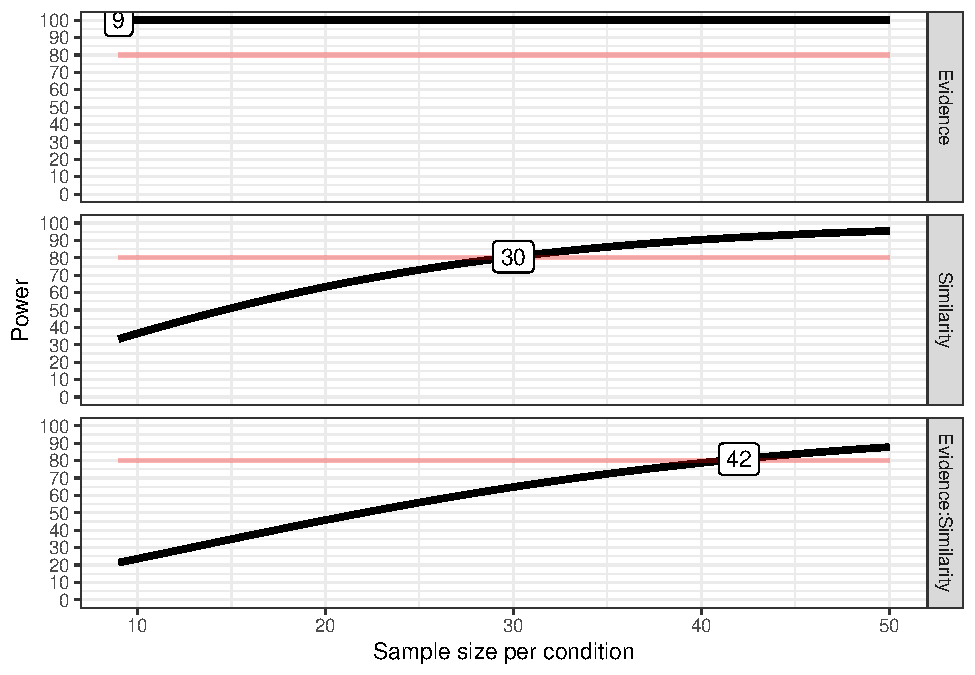
\includegraphics[width=1\linewidth]{anecdotal-bias-in-allocation-decisions_files/figure-latex/power-analysis-1-1} \caption{Power curves for the similarity and anecdote effects.}\label{fig:power-analysis-1}
\end{figure}

\hypertarget{instructions-materials-1-appendix}{%
\subsection{Instructions}\label{instructions-materials-1-appendix}}

Figure~\ref{fig:general-instructions-1} shows the general
instructions all participants received, and
Figures~\ref{fig:specific-instructions-anecdote-only-1},~\ref{fig:specific-instructions-combined-1},~\ref{fig:specific-instructions-enhanced-1},
and~\ref{fig:specific-instructions-statistics-only-1} show
the condition-specific instructions.



\begin{figure}
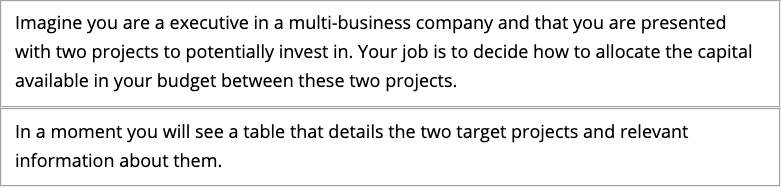
\includegraphics[width=1\linewidth]{anecdotal-bias-in-allocation-decisions_files/figure-latex/general-instructions-1-1} \caption{Experiment~1 general instructions. The two boxes were split between two separate web-pages.}\label{fig:general-instructions-1}
\end{figure}



\begin{figure}
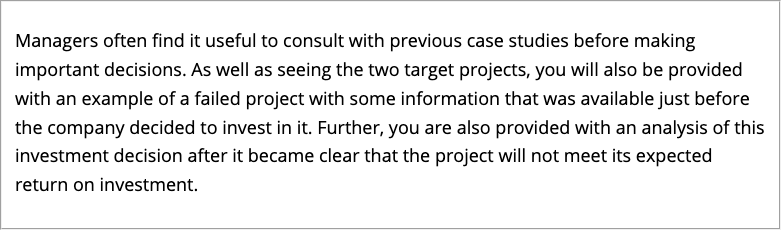
\includegraphics[width=1\linewidth]{anecdotal-bias-in-allocation-decisions_files/figure-latex/specific-instructions-anecdote-only-1-1} \caption{Experiment~1 specific instructions for those in the anecdotes only condition.}\label{fig:specific-instructions-anecdote-only-1}
\end{figure}



\begin{figure}
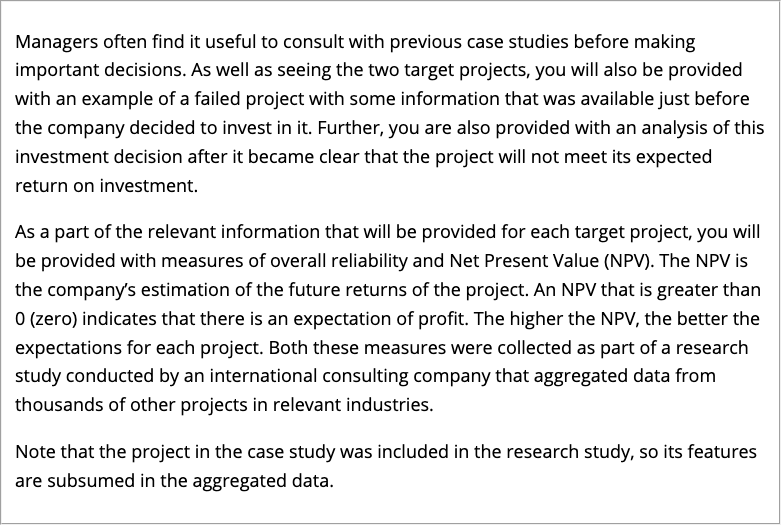
\includegraphics[width=1\linewidth]{anecdotal-bias-in-allocation-decisions_files/figure-latex/specific-instructions-combined-1-1} \caption{Experiment~1 specific instructions for those in the anecdote \& statistics condition.}\label{fig:specific-instructions-combined-1}
\end{figure}



\begin{figure}
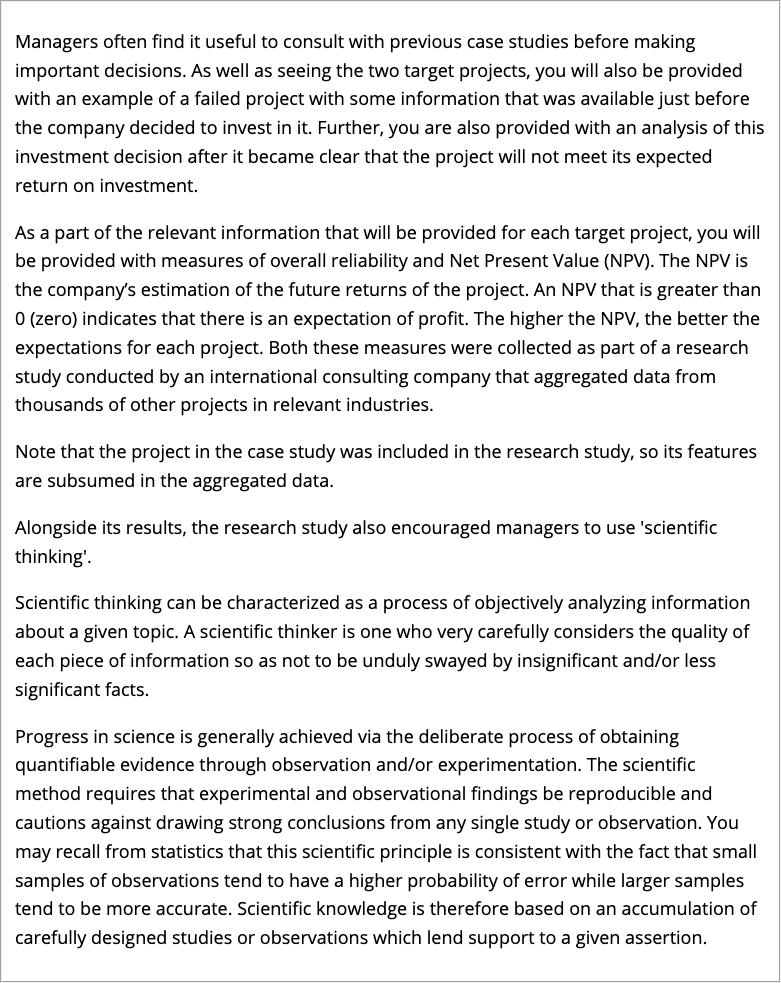
\includegraphics[width=1\linewidth]{anecdotal-bias-in-allocation-decisions_files/figure-latex/specific-instructions-enhanced-1-1} \caption{Experiment~1 specific instructions for those in the anecdote \& enhanced statistics condition.}\label{fig:specific-instructions-enhanced-1}
\end{figure}



\begin{figure}
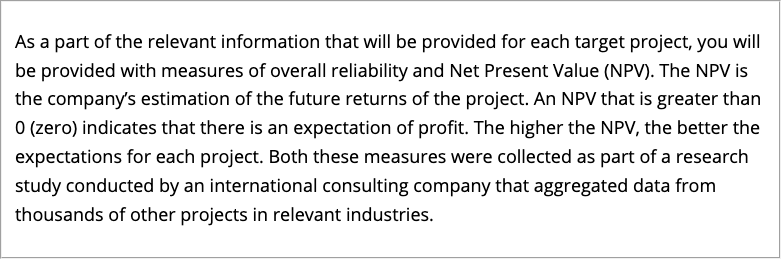
\includegraphics[width=1\linewidth]{anecdotal-bias-in-allocation-decisions_files/figure-latex/specific-instructions-statistics-only-1-1} \caption{Experiment~1 specific instructions for those in the statistics only condition.}\label{fig:specific-instructions-statistics-only-1}
\end{figure}

\hypertarget{follow-up-materials-1}{%
\subsection{Follow-up}\label{follow-up-materials-1}}

Figure~\ref{fig:follow-up-1} shows the follow-up questions.



\begin{figure}
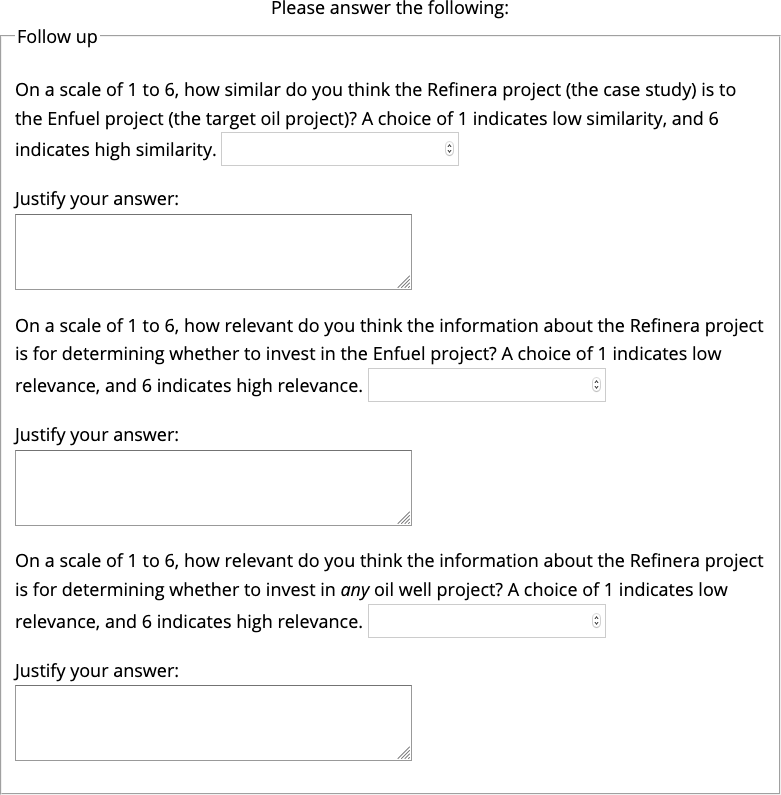
\includegraphics[width=1\linewidth]{anecdotal-bias-in-allocation-decisions_files/figure-latex/follow-up-1-1} \caption{Follow-up questions in Experiment~1.}\label{fig:follow-up-1}
\end{figure}

\hypertarget{experiment-2}{%
\section{Experiment 2}\label{experiment-2}}

\hypertarget{hypothesised-effects-anecdotes-2}{%
\subsection{Hypothesised Effects}\label{hypothesised-effects-anecdotes-2}}

Figures~\ref{fig:plot-simulation-2-negative}
and~\ref{fig:plot-simulation-2-positive} show the simulated data for
the negative and positive valence conditions, respectively. These figures are
different from the equivalent figures in the main text. Here, the same
statistics only value was used for both valence conditions, whereas in the main
text the relevant values for each condition were used. Further, the main text
reports the difference score from the relevant statistics only values, whereas
here the raw means are shown.



\begin{figure}
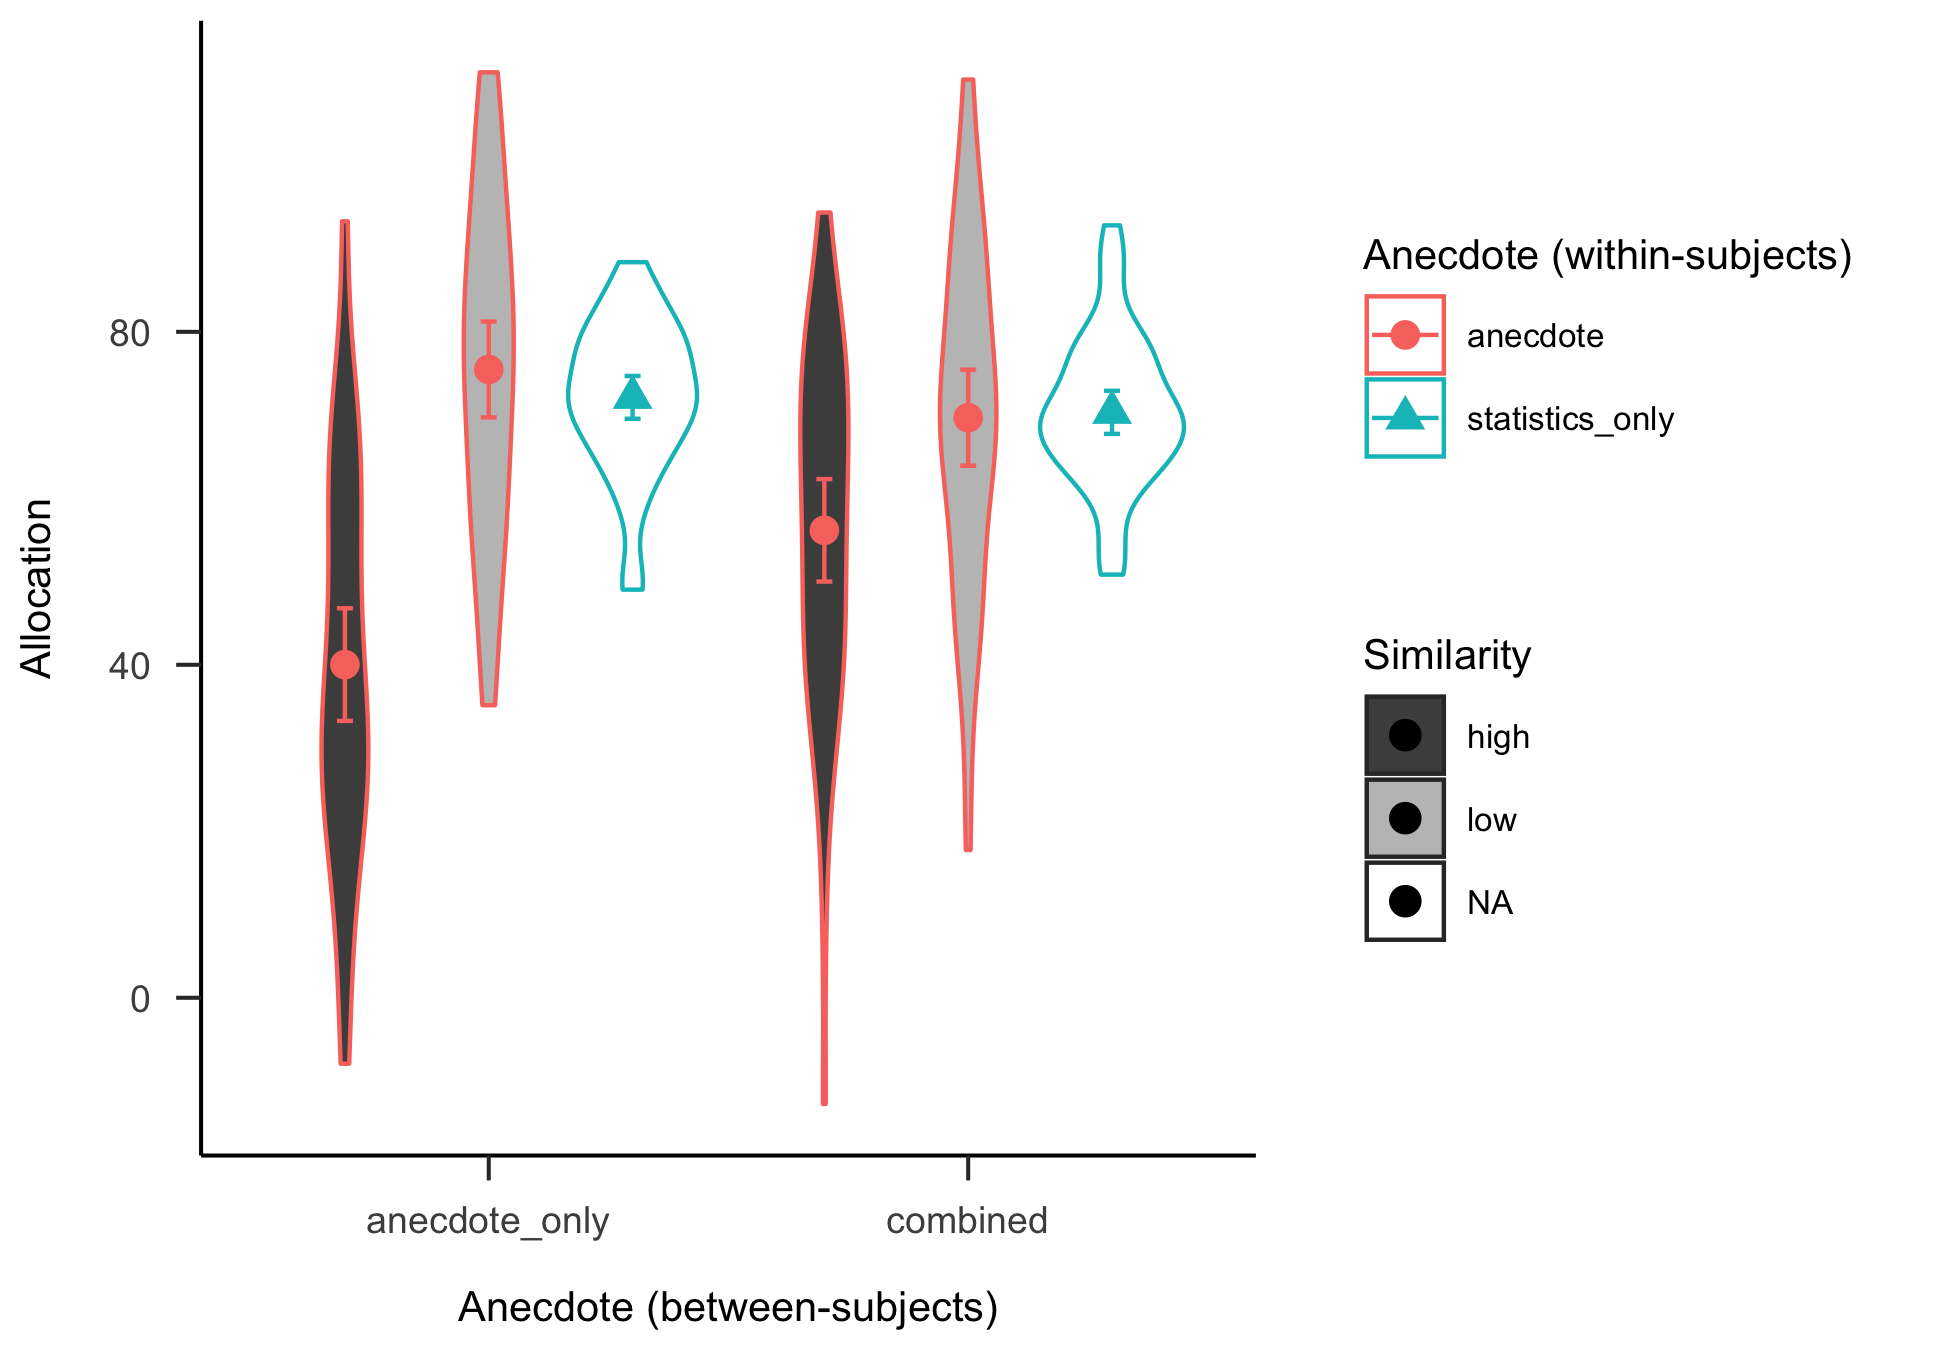
\includegraphics[width=1\linewidth]{anecdotal-bias-in-allocation-decisions_files/figure-latex/plot-simulation-2-negative-1} \caption{Anecdotes Experiment~2 predicted data for the negative valence condition}\label{fig:plot-simulation-2-negative}
\end{figure}



\begin{figure}
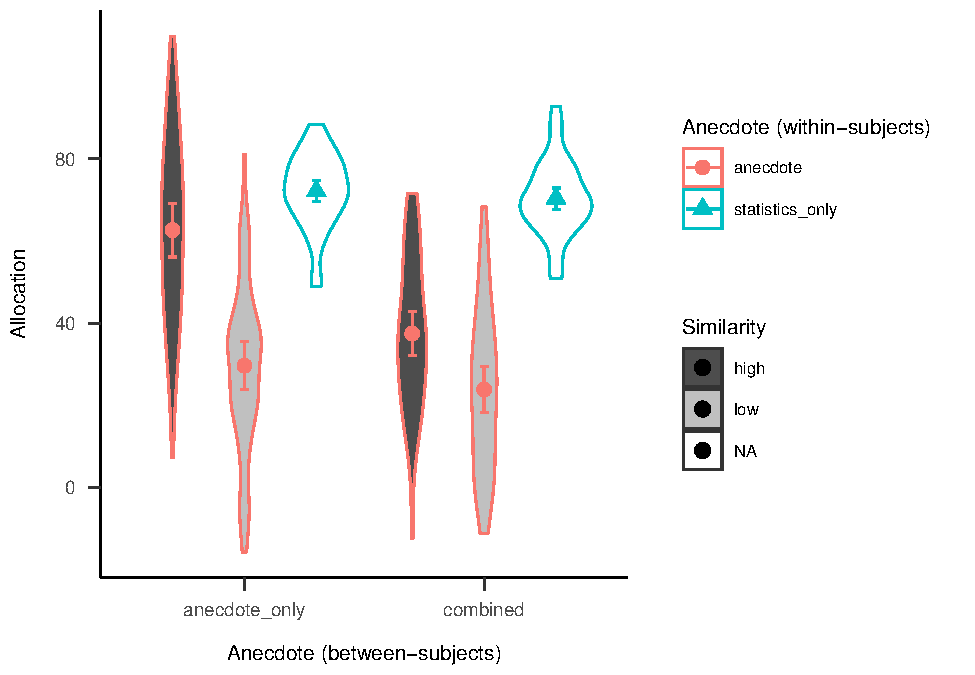
\includegraphics[width=1\linewidth]{anecdotal-bias-in-allocation-decisions_files/figure-latex/plot-simulation-2-positive-1} \caption{Anecdotes Experiment~2 predicted data for the positive valence condition}\label{fig:plot-simulation-2-positive}
\end{figure}

\hypertarget{power-analysis-2}{%
\subsection{Power Analysis}\label{power-analysis-2}}

A power analysis was conducted through simulation of the effects implied by the
hypotheses in Experiment~2. Data were simulated with the same mean values as
Experiment~1 for the effects that were previously significant (i.e., similarity,
statistics, and interaction effects), and no effect for the differences that
were non-significant (as shown in
Figures~\ref{fig:plot-simulation-2-negative}
and~\ref{fig:plot-simulation-2-positive}). The null effect was
analysed using the two one-sided tests (TOST) procedure, or \emph{equivalence}
testing (\protect\hyperlink{ref-lakens2018}{Lakens et al., 2018}), and setting the smallest effect size of interest to the
smallest difference that leads to a significant equivalence between the combined
low similarity and statistics only conditions in Experiment~1.
Figure~\ref{fig:power-analysis-2} shows the results of this analysis,
which suggested a total sample size of 92
(46 \(\times\) 2).

\newpage

\begin{landscape}



\begin{figure}
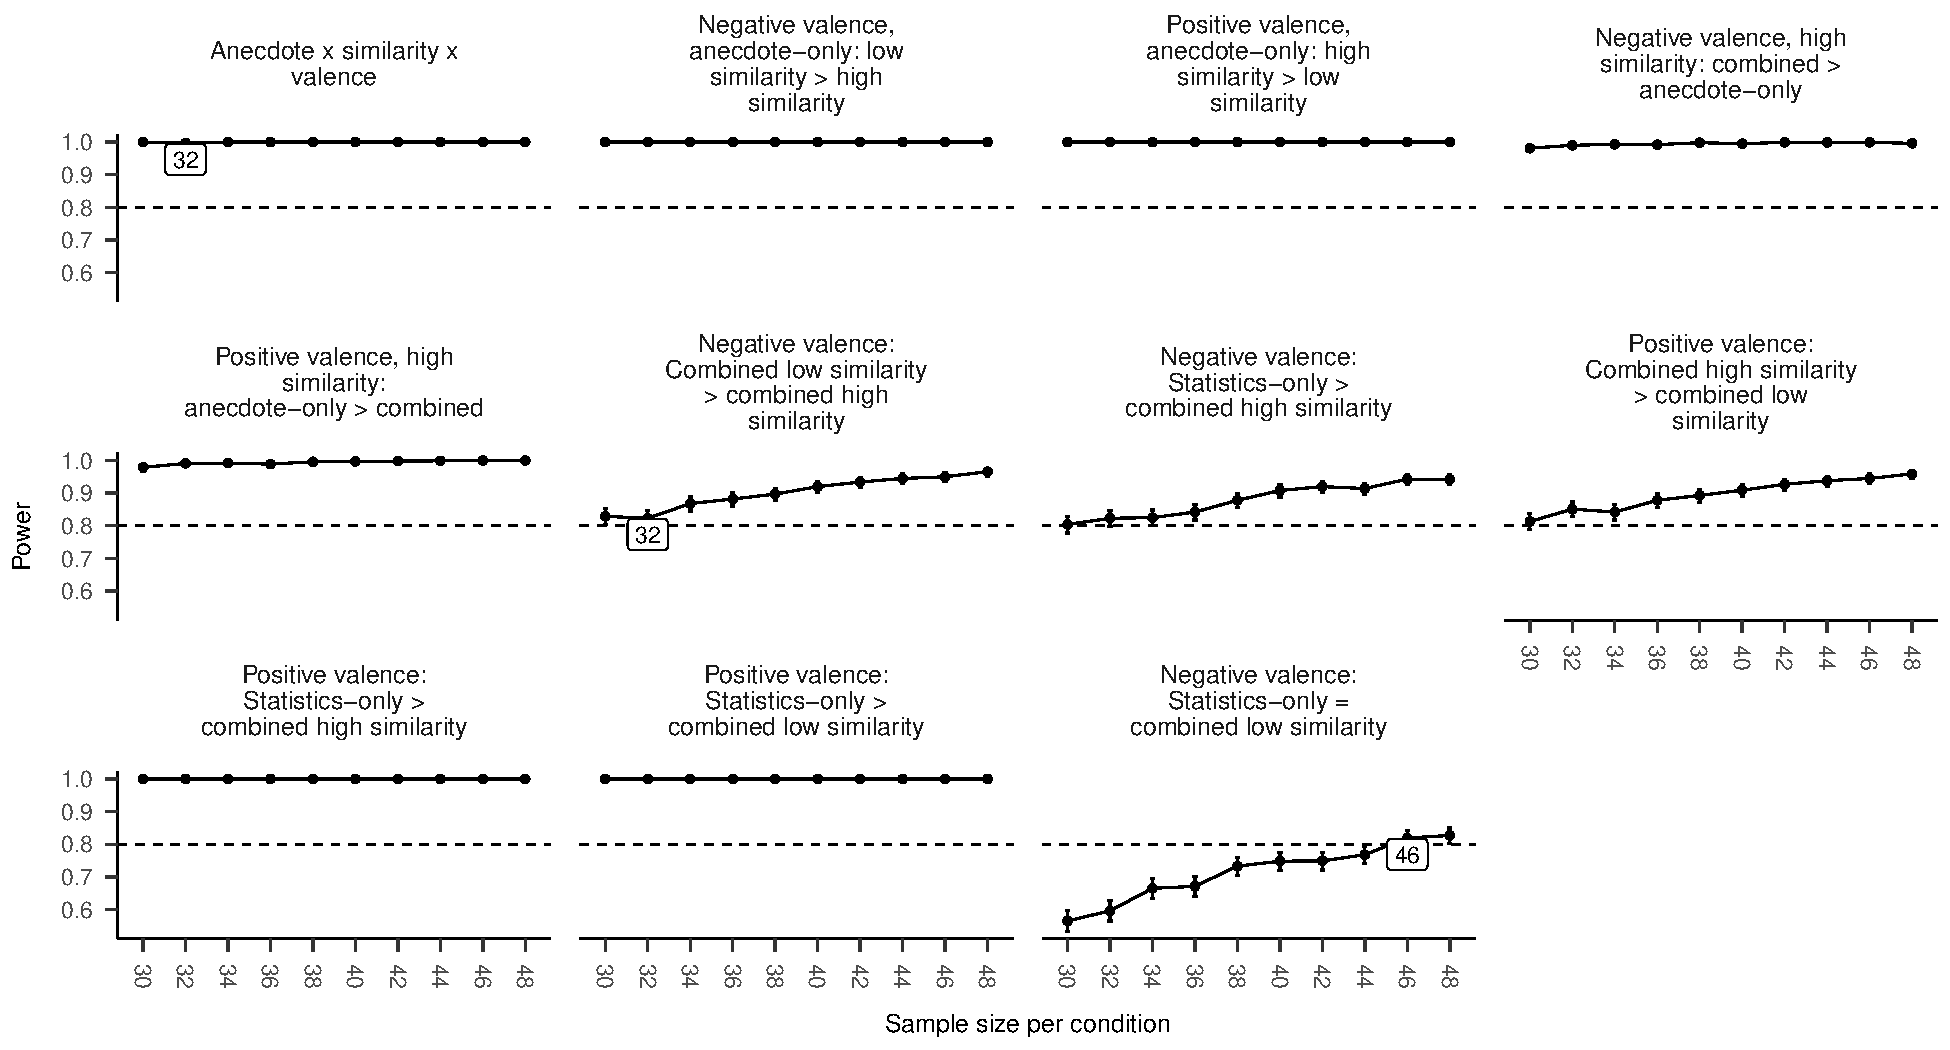
\includegraphics[width=1\linewidth]{anecdotal-bias-in-allocation-decisions_files/figure-latex/power-analysis-2-1} \caption{Anecdotes Experiment~2 power curve. Labels indicate lowest sample size above 80\% power.}\label{fig:power-analysis-2}
\end{figure}

\end{landscape}

\newpage

\hypertarget{instructions-materials-2-appendix}{%
\subsection{Instructions}\label{instructions-materials-2-appendix}}

Figure~\ref{fig:general-instructions-2} shows the general
instructions all participants received, and
Figures~\ref{fig:specific-instructions-anecdote-only-2},~\ref{fig:specific-instructions-combined-2},
and~\ref{fig:specific-instructions-statistics-only-2} show
the condition-specific instructions.



\begin{figure}
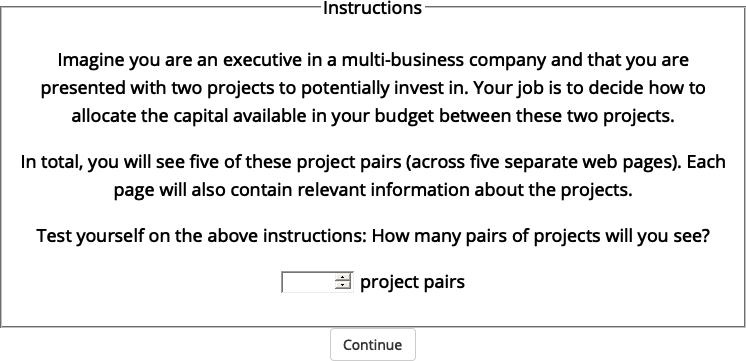
\includegraphics[width=1\linewidth]{anecdotal-bias-in-allocation-decisions_files/figure-latex/general-instructions-2-1} \caption{General instructions for Experiment~2.}\label{fig:general-instructions-2}
\end{figure}



\begin{figure}

\includegraphics[width=1\linewidth]{anecdotal-bias-in-allocation-decisions_files/figure-latex/specific-instructions-anecdote-only-2-1} \caption{Experiment~2 specific instructions for those in the anecdotes only condition.}\label{fig:specific-instructions-anecdote-only-2}
\end{figure}



\begin{figure}

\includegraphics[width=1\linewidth]{anecdotal-bias-in-allocation-decisions_files/figure-latex/specific-instructions-combined-2-1} \caption{Experiment~2 specific instructions for those in the combined condition.}\label{fig:specific-instructions-combined-2}
\end{figure}



\begin{figure}

\includegraphics[width=1\linewidth]{anecdotal-bias-in-allocation-decisions_files/figure-latex/specific-instructions-statistics-only-2-1} \caption{Experiment~2 specific instructions for those in the statistics only condition.}\label{fig:specific-instructions-statistics-only-2}
\end{figure}

\hypertarget{follow-up-materials-2}{%
\subsection{Follow-up Questions}\label{follow-up-materials-2}}

Figure~\ref{fig:follow-up-2} shows an example of the
follow-up questions.



\begin{figure}
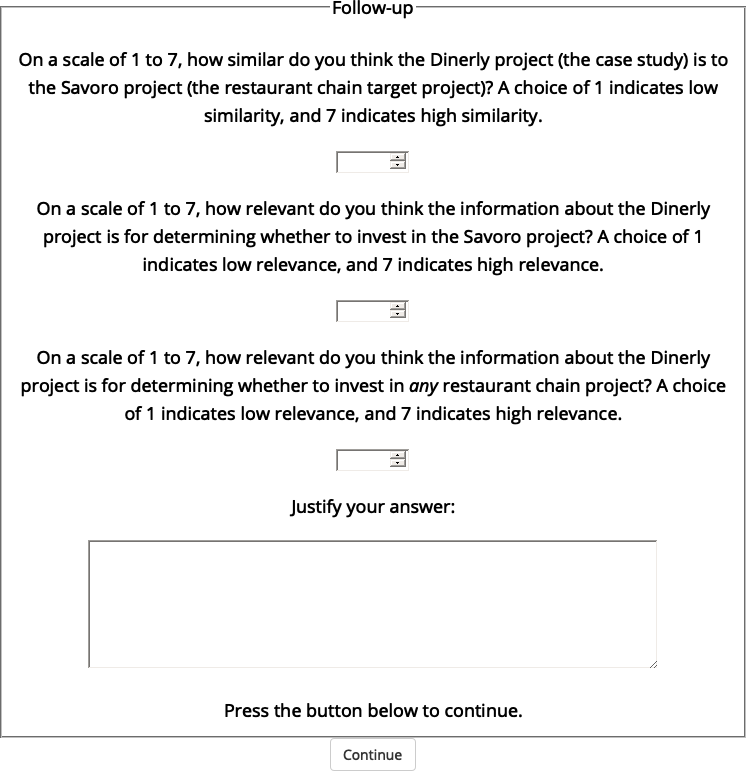
\includegraphics[width=1\linewidth]{anecdotal-bias-in-allocation-decisions_files/figure-latex/follow-up-2-1} \caption{An example of one of the follow-up question displays in Experiment~2.}\label{fig:follow-up-2}
\end{figure}

\hypertarget{interstitial-materials-2}{%
\subsection{Interstitial Display}\label{interstitial-materials-2}}

Figure~\ref{fig:interstitial-2} shows an example of one of
the interstitial displays.



\begin{figure}
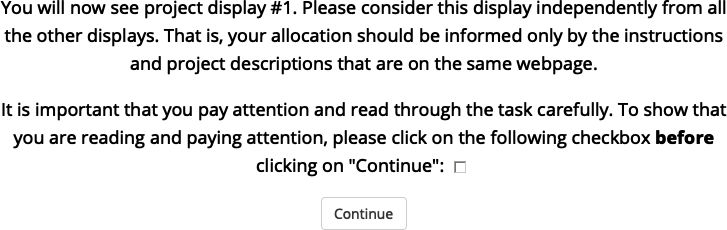
\includegraphics[width=1\linewidth]{anecdotal-bias-in-allocation-decisions_files/figure-latex/interstitial-2-1} \caption{An example of an interstitial display in Experiment~2.}\label{fig:interstitial-2}
\end{figure}

\hypertarget{results-2-appendix}{%
\subsection{Similarity Manipulation Check}\label{results-2-appendix}}

The similarity manipulation worked as expected, with the negative anecdote only
low similarity condition being allocated significantly more than those in the
high similarity condition,
\(\Delta M = 26.98\), 95\% CI \([17.99, 35.97]\), \(t(94) = 5.96\), \(p < .001\). For
positive anecdotes, participants allocated more to the high similarity condition
than those in the low similarity condition,
\(\Delta M = 22.63\), 95\% CI \([13.79, 31.46]\), \(t(94) = 5.08\), \(p < .001\). Evidence
for the similarity manipulation working was also seen in the rating data.
Participants rated anecdotes in the high similarity condition as more similar to
the target than those in the low similarity condition,
\(F(1, 94) = 48.36\), \(p < .001\), \(\hat{\eta}^2_p = .340\).


\end{document}
